% !TEX TS-program = xelatex
% !TEX encoding = UTF-8 Unicode

\documentclass[hidelinks, 12pt]{article} % Use larger type; default is 10pt
\linespread{1.5}
\usepackage[utf8]{inputenc} % Set input encoding (not needed with XeLaTeX)
\usepackage[x11names]{xcolor} % Enables the use of custom colors
\usepackage{amsmath, amssymb, array, booktabs, multirow, makecell, bigdelim, pdflscape, placeins, hvfloat, longtable, rotating, pdfpages, textcomp, fancyhdr, graphicx, float, upgreek, gensymb, hyperref}
\usepackage[nottoc,notlof,notlot]{tocbibind} % Include bibliography in ToC
\usepackage[most]{tcolorbox} % For coloured information boxes
% Define your custom color
\definecolor{customcolor}{HTML}{F1EEE2}

\usepackage[titles,subfigure]{tocloft} % Customize ToC style
\usepackage{titletoc, sectsty, soul} % Formatting for ToC and sections
\usepackage[super]{nth}
\usepackage[OT1]{fontenc}
\PassOptionsToPackage{hyphens}{url}
\usepackage{geometry} % Ensure the geometry package is loaded
\geometry{a4paper, total={170mm,257mm}, left=20mm, top=20mm}

\usepackage{fontspec} % Required for custom fonts
\usepackage{unicode-math}
\usepackage{amsmath, amssymb}



% For pdflatex:
% Use cmvtt for text and math
% Set text to cmvtt font
% \renewcommand*\ttdefault{cmvtt}
% % \renewcommand*\ttdefault{qcr}
% \renewcommand*\familydefault{\ttdefault}
% \usepackage[T1]{fontenc}
% % Define math font commands to mimic cmvtt

% \DeclareMathAlphabet{\mathcmtt}{OT1}{cmtt}{m}{n}
% % Command for math in typewriter font
% \newcommand{\ttmath}[1]{{\mathcmtt{#1}}}


% For xelatex:
\setmainfont{Harding Text Web} % Main document font
\setmathfont{Harding Text Web}

% Define a math font face for Marcellus
\setmathfontface\mathmarcellus{Harding Text Web}

% Define the \ttmath command for math mode using Marcellus
\newcommand{\ttmath}[1]{{\mathmarcellus{#1}}}






% Custom commands
\newcommand{\ddfrac}[2]{\frac{\displaystyle \raisebox{0.5ex}{$#1$}}{\displaystyle \raisebox{-0.5ex}{$#2$}}}
\newcommand{\dddfrac}[2]{\frac{\displaystyle \raisebox{1ex}{$#1$}}{\displaystyle \raisebox{-1ex}{$#2$}}}
\newcommand{\bsk}{\vspace{\baselineskip}}
\newcommand{\myline}{\par\noindent\makebox[\linewidth]{\rule{\textwidth}{0.4pt}}}
\newcommand{\subsubsubsection}[1]{\paragraph{#1}\mbox{}}

% Headers & Footers
\pagestyle{fancy}
\fancyhf{}
\fancyfoot[C]{\thepage}
\renewcommand{\headrulewidth}{0pt}

\fancypagestyle{lscape}{%
  \fancyhf{}
  \fancyfootoffset[R]{-50cm}
  \fancyfoot[R]{\makebox[0pt][r]{\rotatebox{90}{\thepage}}}
  \renewcommand{\headrulewidth}{0pt}
  \renewcommand{\footrulewidth}{0pt}}

% Customize Table of Contents
\renewcommand{\cftsecfont}{\normalfont\bfseries}        % Section font (normal + bold)
\renewcommand{\cftsecpagefont}{\normalfont\bfseries}    % Page number font (bold)
\renewcommand{\cftsubsecfont}{\normalfont\itshape}      % Subsection font (italic)
\renewcommand{\cftsubsecpagefont}{\normalfont\itshape}  % Subsection page number font

% Adjust spacing in the ToC
\setlength{\cftbeforesecskip}{1em}   % Spacing before section entries
\setlength{\cftbeforesubsecskip}{0.5em} % Spacing before subsection entries

% Section numbering
\setcounter{secnumdepth}{4}
\setcounter{tocdepth}{4}

% Document content
\title{
  \vspace{-1cm}
  \textbf{Uncovering Hidden Carbon Reservoirs:\\
  The geochemistry of Himalayan groundwaters}
  \vspace{0.5cm}
}
\author{Giovanni Bernardi}
\date{2024-2025}



\begin{document}
%\justifying
% \raggedright

\maketitle





\thispagestyle{empty}

\newpage

\section*{Abstract}
\label{sec:abstract}
\addcontentsline{toc}{section}{\nameref{sec:abstract}}

This is the abstract. Feel free to add anything insightful... or not :). Hello!


\pagenumbering{roman}

\newpage


\thispagestyle{empty}
%need to change this to the main report font

\tableofcontents

\newpage

\thispagestyle{empty}

\section*{Acknowledgements}

\newpage

\thispagestyle{empty}

\section*{List of Tables}

\newpage

\thispagestyle{empty}

\section*{Nomenclature}
%\thispagestyle{empty}

\newpage

\pagenumbering{arabic}



\FloatBarrier
\pagenumbering{arabic}




\section{Introduction}
%%SHARP SCIENTIFIC LANGUAGE


% WHAT IS THE PROBLEM?
\subsection{Project Outline}

Silicate weathering, whereby silicate minerals are dissolved by carbonic acid, 
sequesters atmospheric CO$_2$ over long (10$^5$ year) timescales, influencing global climate regulation.
The Himalayan mountain range spans more than 590,000 km$^2$, and is the source of major rivers, including the Ganges, Brahmaputra, and Indus. 


\bsk

In highly erosive regions where the supply of silicate minerals far exceeds the weathering rate, silicate weathering reactions are thought to be sensitive to climate (Stallard \& Edmund 1983 JGR, West et al, 2005) The dissolution kinetics of the largely silicate rocks in these catchments are sensitive to temperature and runoff because the weathering reactions have not gone to completion. Silicate weathering in the Himalayas as a result of their uplift and erosion in the Cenozoic may have contributed significantly to the global 
cooling over the past 40 million years %[reword] 
(Raymo and Ruddiman, 1992; West et al, 2005, Kump et al, 2000 Ann Rev Earth Sci). 
Thus, it is this sensitivity to climate as well as their large size that makes them important to study, from both a scientific and practical perspective. More recent models have proposed silicate weathering is more sensitive to the hydrological cycle, than to temperature [cite]. There are a range of flow paths with different residence times, and rock is exhumed through these flow paths with a much longer time constant than the water in the flow paths.

\bsk

However, there remain a number of unknowns in the weathering fingerprints of these catchments, namely the residence time of the water,
flow path direction and length, rate of reaction, and extent to which equilibrium is reached.
Understanding residence time in particular is important because the geochemical reactions that are used to quantify weathering 
(and the biogeochemical ones too) are time-dependent.
Residence time will also reflect the variety of flow routes within a catchment, and help to constrain hydrological models. In this contribution the flow paths and residence times of water will be investigated using the chemical weathering products of spring waters from a highly monitored Himalayan catchment. This will not only provide better constraints on reaction rates of silicate mineral dissolution reactions in the field, but also a greater understanding of the role of hydrology in providing a climate-sensitive negative feedback between atmospheric CO$_2$ and silicate mineral dissolution
An added benefit will also be provided via a greater understanding of Himalayan water supplies which are essential for billions of people (Ives and Messerli, 1989). 

%can always pinch from this and write to abstract
    
\newpage

\begin{tcolorbox}[
    colback=customcolor, % Use the defined custom color for background
    colframe=white,      % Set the frame color to white (invisible)
    sharp corners,       % Straight edges
    boxrule=0pt,         % No border width
    breakable,           % Allow the box to break into multiple pages (if needed)
    width=\dimexpr\textwidth+2cm\relax, % Make the box wider than \textwidth
    enlarge left by=-1cm,   % Shift box left to center the extra width
    leftrule=0mm,        % No left border
    rightrule=0mm,       % No right border
    toprule=0mm,         % No top border
    bottomrule=0mm       % No bottom border
]
\textbf{\Large Box 1}
\vspace{-3mm}
\myline\\
\textbf{\Large Chemical Weathering}
\vspace{-3mm}
\myline\\
{\footnotesize
As water passes through the subsurface, it interacts with rock. This causes the addition of solute species to water, and the formation of stable secondary minerals through the dissolution of primary minerals formed at different pressure and temperature. Dissolved CO$_2$ derived from the atmosphere present in rainfall makes it slightly acidic. This acidity is further increased by the presence of decomposition of organic matter and CO$\ttmath{_2}$ production from organic activity in the soil.
\[
\ttmath{H_2O + CO_2 \rightarrow H_2CO_3 \rightarrow HCO_3^- + H^+}
\]

Carbonic Acid Weathering of Carbonate - Net Zero
    
    \begin{center}
    
    Short Term [timescale]:
    \[
    \ttmath{CaCO_3 + CO_2 + H_2O = Ca^{2+} + 2HCO_3^-}
    \]
    
    Long Term [timescale]:
    \[
    \ttmath{Ca^{2+} + 2HCO_3^- = CaCO_3 + CO_2 + H_2O}
    \]

    \end{center}
    
    
Carbonic Acid Weathering of Silicate - Net CO$\ttmath{_2}$ drawdown

    \begin{center}

    Short Term [timescale]:
    \[
    \ttmath{2CO_2 + 3H_2O + CaAl_2Si_2O_8 = Ca^{2+} + 2HCO_3^- + Al_2Si_2O_5(OH)_4}
    \]
    
    Long Term [timescale]:
    \[
    \ttmath{Ca^{2+} + 2HCO_3^- = CaCO_3 + CO_2 + H_2O}
    \]
    
    \end{center}

The rate of weathering is dependent on the mineralogy of the rock. Different minerals weather at different rates (from Shand et al, 1999: quartz > albite > mafic silicates > anorthite > carbonates), so the most reactive minerals will contribute disprportionately to the solute load of the water. [Something about Tipper 2006 and carbonates during monsoon?? somewhere]. Note that here, only the weathering of carbonic acid is considered. Sulfuric acid is also often considered a big player in weathering, but its impact is not considered in this study because the pyrite deposits required for its formation are not present in lithological studies of the Melamchi region [follow up].
\[
\ttmath{4FeS_2 + 15O_2 + 14H_2O \rightarrow 4Fe(OH)_3 + 8H_2SO_4}
\] 

Mineral reactions are also time-dependent, so the longer that water spends in contact with the rock, the higher the degree of completion of a chemical reaction [can mention incongruent dissolution whereby only part of the mineral dissolves?]. Current models of silicate and carbonate weathering (the two dominant lithologies considered) do not generally consider underground flow paths in their carbon flux estimates (Gaillardet et al, 1999 and others). Hence, a potentially underestimated part of the carbon cycle is this underground weathering.

}
\end{tcolorbox}


\newpage

%\section{Literature Review}



% DISSOLUTION RATES:

% \item{Kump et al, 2000: The relative rates of dissolution of silicate minerals are similar in field and laboratory but they differ by orders of magnitude. Chemical erosion rates are dependent on how intense the hydrological cycle is}

% \item{White and Brantley, 2003: Field conditions are different to lab conditions. Processes "extrinsic" to the weathering conditions cannot be replicated in the lab}

% \item{Kampman et al, 2009: Correlation between delta G and rate of reaction when comparing lab and field rates - they plot in different places, the field ones being closer to equilibrium.}

% \item{West et al, 2005: } - BRIDGE

% CONTROLS ON WEATHERING - LINK FROM West:

% \item{Stallard and Edmond, 1983: Geological variations lead to differences in soil composition, landscape features, vegetation, and climate. Topography also influences soil properties. The contribution of weathering from different lithologies should be proportional to their area within the catchment.}

% \item{Pedrazas et al, 2021: Describe two weathering fronts, shallow with extensive fracturing and deep with open fractures. Weathering fraction scales with hillslope length}

% \item{Singh et al, 1987: Increase in porosity for the same decrease in density for sanstone > porphyritic gneiss > quartzite > pegmatite > amphibolite > biotite gneiss > basalt > dolerite}

% \item{Marques et al, 2009: Porosity increases as the rock becomes more weathered, as does the water content. Maybe you can put their weathering index there}

% \item{David et al, 1994: Low porosity rock have porosity less than 5\%. High porosity rocks have porosity greater than 15\%. Relationship between permeability and porosity and depth is exponential, link to Mike}

% \item{Gaillardet et al, 1999: 60 largest rivers in the worlkd. Aims to fit an inverse model looking at silicate weathering for Co2 consumption. bickle on why inverse models do not work.... Carbonate weathering has no effect over million year timescales on atmospheric CO2. low Ca/Na molar ratios are expected in dissolved load of rivers draining silicates }

% \item{Medwedeff et al, 2021: Weathering controls shallow bedrock strength more so than mineral or textural differences between the metamorphic lithologies. Weathering also varies systematically with vegetation and topography. Weathering decreases above the tree line (though we do not have data for this).}


% PRECIPITATION EFFECTS:

% \item{Andermann et al. (2012) show that anticlockwise hysteresis loops of precipitation against discharge (include basic schematic) suggest that there is a 3 month lag in the response of the river to precipitation.  The delay in river discharge is a topic of debate. Andermann et al. (2012) propose that at lower elevations, it is more likely due to groundwater storage of precipitation in the fractured basement}

% \item{Bookhagen and Burbank (2010) suggest that the delay of precipitation and discharge may be due to the response of glaciers at higher elevations. They also suggest evaportranspiration has a low impact on the hydrological budget of the Himalayas, less than 10\%.}

% \item{McGuire et al, 2005: Catchments with little glacial input show the same delay. Residence time of groundwater can hence be used to quantify this delay and nature of its origin}


\subsection{Lithological controls on weathering}

Differences in lithology are thought to affect weathering. Geological differences lead to differences in soil composition, landscape features, vegetation, and climate which in turn affect the rates of reaction. Logically, the contribution of one lithology to weathering is correlated to its spatial extent in the catchment (Stallard and Edmond, 1983). Porosities vary widely across a catchment depending on the rock type encountered (Singh et al, 1987; David et al, 1994). Porosity also increases as a rock becomes more weathered (Marques et al, 2009). Weathering regimes can be classified as either transport-limited or kinetically limited (West et al., 2005). West et al. distinguish the two regimes by the rate of erosion in the catchment. In low erosion rate settings, weathering is transport-limited due to limited mineral supply. Weathering here is therefore proportional to the material eroded. In high erosion rate settings, weathering is kinetically limited due to an abundant mineral supply. Rapidly eroding catchments like Melamchi are therefore likely kinetically limited. Soil properties and topography are used to identify different "weathering regimes" in the subsurface (Pedrazas et al, 2021). Indeed, bedrock strength is thought to be more dependent on weathering than mineral or textural differences between the metamorphic lithologies in the Himalayas (Medwedeff et al, 2021).

\subsection{Dissolution rate findings}

There is general consensus in the scientific community that rates of dissolution of minerals are different depending on whether they are measured in the field or in a laboratory. White and Brantley (2003) explain this difference by denoting 'extrinsic' qualities that are variable in the field, such as permeability and mineral/fluid ratios. The rate of dissolution of a mineral has also been linked to the free energy of the system, with laboratory rates being calculated significantly more far away from equilibrium (a higher delta G) than field rates (Kampman et al, 2009). This implies that field localities are closer to equilibrium than laboratory-derived rates might suggest. Add Maher et al, 2009 and why they think lab and field are different.

\subsection{Response to monsoonal precipitation}
What makes the Himalayas unique is also what makes them difficult to model, namely the monsoon. This is characterised by a strong seasonal reversal of winds, which brings heavy rainfall to the region during the summer months, and dry conditions during the winter (Bookhagen and Burbank, 2010). The monsoon brings a large amount of precipitation to the region. Andermann et al. (2012) show that anticlockwise hysteresis loops of precipitation against discharge (include basic schematic) suggest that there is a 3 month lag in the response of the river to precipitation.  The delay in river discharge is a topic of debate. Andermann et al. (2012) propose that at lower elevations, it is more likely due to groundwater storage of precipitation in the fractured basement. Bookhagen and Burbank (2010) suggest that the delay of precipitation and discharge may be due to the response of glaciers at higher elevations. They also suggest evaportranspiration has a low impact on the hydrological budget of the Himalayas, less than 10\%. Other studies have found that catchments with little glacial input show the same delay, suggesting that the former hypothesis may be more relevant to this discussion (McGuire et al, 2005). The residence time of groundwater can hence be used to quantify this delay and nature of its origin.



% PRECIPITATION AND CLIMATE:

% \item{Acharya et al, 2020: Higher elevations during the monsoon receive lots of water from the southerly winds rather than from the westerlies. Makes sense. Also suggests most of the water input comes from the top quarter or so of the catchment.}

% \item{Wen et al, 2012: Southern Himalaya have a large altitude contrast over a short distance. Isotopic lapse rate is smaller in the monsoon season and higher in the non monsoon seasonl, implying a role of the monsoon precipitation in the lower lapse rate}

% \item{Kattel et al, 2012: They can model the lapse rate in the Himalayas. The large range in altitude clearly leads to a large spatial variation in temperature. Climate in Nepal is tropical to alpine in s very short x-y distance. They state that the foothill slopes of the Himalayas receive the most rain, which disagrees with Acharya et al, 2020.}

% \item{Panthi et al, 2015: The arrival date for the monsoon in Nepal has not changed bu the withdrawal is getting later. Precipitation is more intense on a per day basis. This is bad for the crops in winter season because of lack of moisture and obviously causes more disasters and floods} LINK TO DISASTER

% \item{Baniya et al, 2012: Flooding in Melamchi in 2021: precipitation is the main climatic driver of flooding, and increasing temperature leads to higher magnitude floods} LINK TO DISASTER



% DISASTER EFFECTS:

% \item{Graf et al, 2023: the 2015 Gorkha EQ changed the geomorphology of the Melamchi catchment. The landslides that followed contributed significantly to the 13 milliom m3 sediment deposited during the later 2021 Melamchi flood. The EQ was important but only tipped an already unstable system.}

% The monsoon brings a large amount of water in the form of precipitation to the region, which reacts with the CO$_2$ in the air to make carbonic acid. This subsequently reacts and dissociates with the silicate minerals, drawing down atmospheric CO$_2$ (see some section with the full equations). [Something about Illien and how it is linked to groundwater flow]


\subsection{Study aims}

% WHAT DOES THIS STUDY DO?

In the present study, spring and rain samples from the Melamchi catchment are used as a case 
study to investigate the weathering rates in a rapidly eroding catchment. The sample dataset consists of 372 samples spanning four field campaigns over three years (2021-2024), as well as more recent year-long bi-weekly timeseries data from stream and spring samples in sites across the catchment. [See map] 
As Tipper et al, 2006 writes, studying small catchments gives the opportunity to attribute large changes in water chemistry to seasonal climate changes like the monsoon. (More in Area)


% \item WHAT DOES THIS STUDY SHOW IN THEIR RESULTS? % \item WHAT HAVE PREVIOUS MODEL STUDIES SHOWN?
 
\bsk

This study considers major and trace ion concentrations, alkalinity, and radiogenic strontium isotopes from the Melamchi catchment. This study shows that there are systematic variations in the chemical composition of the water along and away from the ridge. These can be explained through lithological differences and chemical weathering respectiuvely. Estimation of the carbon flux in the groundwater yields ******?. Residence time calculations determined using rate constants close to equilibrium give ages of 10-25 years. This is in agreement with previous studies which calculated residence times using gas ages (Atwood et al [expand on this]). Previous studies have linked residence time to topography, such that areas with a small topographic gradient evolve to a larger residence time and vice versa. (McGuire et al, 2005). A similar relationship is found in this study.

 
\bsk
% \item WHAT ARE WE DOING DIFFERENTLY? WHAT ARE THE ADVANTAGES OF DOING THIS DIFFERNTLY?

So far, papers modelling the evolution of weathering have not considered catchment-based data due to the non-ideal setting. This study aims to bridge that gap by applying simplified models to a highly monitored catchment. The hope is that this approach will help to give a first-order estimation on parameters that are not easily obtained with the chemistry of a system alone. This report aims to join together studies looking at the same problem from different disciplines.





% \item WHAT ARE THE QUESTIONS WE HOPE TO ANSWER?






% Summary of the key questions (commented):
% 1. What main challenge does this study address?
% 2. What prior work and prevailing perspectives exist?
% 3. What does this investigation aim to accomplish?
% 4. Which results are highlighted by this study?
% 5. How have previous models approached the problem?
% 6. In what ways does this work differ from existing studies?
% 7. Why is this approach potentially more beneficial?
% 8. Which specific questions does this study seek to answer?


\newpage



\section{Study Area}
% Provide a description of the sampling methods, field area, and geology.
% - Include maps or figures if necessary.

% want table with catchment characteristics
% also remember to include a table with abbreviations


The Melamchi-Indrawati catchment (85.441 - 85.601 E, 27.822 - 28.157 N) study area ranges from 790 to 5700 m a.s.l. (metres above sea level). The Melamchi River is a tributary of the larger Indrawati River and runs through the catchment draining an area of 325km$\ttmath{^2}$. 

\subsection{Geology and Geomorphic Setting}

% Need to add Himalayan background

The geology of Melamchi is characterised by the characteristic banded gneiss, feldspathic schist and laminated quartzite of the Higher Himalayan Crystalline Sequence (HHCS). To the south of the confluence of the Melamchi River to its parent Indrawati river lies the Main Central Thrust (MCT) which separates the HHCS from the Lower Himalayan Sequence (LHS) (Dhital et al, Graf et al). The overall geology is therefore largely comprised of silicate metamorphic rock.


\begin{table}[h!]
    \centering
    \begin{small}
    \begin{tabular}{p{3cm} p{1cm} p{1cm} p{1.8cm} p{1.9cm} p{1.5cm} p{3cm}}
           \hline
           \textbf{Catchment} & \textbf{Area} & \textbf{Mean Slope} & \textbf{Mean Elevation} & \textbf{Elevation Range} & \textbf{Geology} & \textbf{Location Range (DD)} \\[4pt]
                              & (km$^2$)    & (\%)                & (m)                     & (m)                      &                &  \\[4pt]
           \hline
           Melamchi Khola     & 325         & 20                  & 2400                    & 786--5697                & HHCS           & 85.441--85.601 E  27.822--28.157 N \\[4pt]
           \hline
    \end{tabular}
    \end{small}
    \caption{Melamchi catchment characteristics. Area, Slope, Elevation data from NASA ASTER (ref). Geology from Dhital et al. (cite).}
    \label{tab:catchment_characteristics}
    \end{table}
    


\subsection{Climate}

Annual mean temperatures in the Melamchi Khola Catchment range from ~24$^{\circ}$C at base elevation to ~8$^{\circ}$C at highest elevation sampled (3200 m a.s.l.). The area is characterised by a high erosion rate.  The southern Himalayas are characterised by a large topographic gradient. This corresponds to a large temperature gradient contributing to tropical and alpine climates close to one another (Kattel et al, 2012). The westerly winds typical of this latitude are responsible for the dry season in the Himalayas (Bookhagen and Burbank, 2010). The source of precipitation during the Indian Summer Monsoon (ISM) affecting Melamchi is the Bay of Bengal, due to the strong pressure gradient that changes the westerly winds to southerly winds. This temperature gradient reverses in the winter, when the oceans are warm and the High Himalaya is cold.  The Melamchi Khola catchment receives over 80\% of its rainfall during the monsoon.

\bsk

Recorded temperatures at the end of the spring flow paths vary with the season, being coldest in November. All seasons show a temperature decrease with increasing elevation, consistent with the free-air moist adiabatic lapse rate, which is = 6.5 $^{\circ}$C/km (Barry and Chorley, 2009).

\begin{figure}[h]
    \centering
    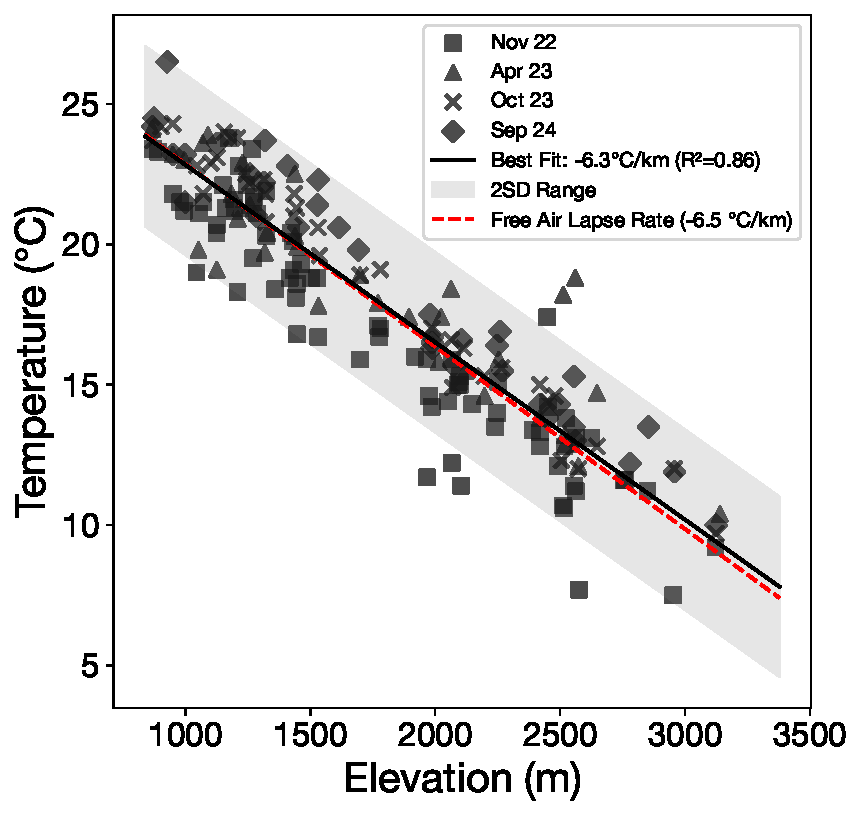
\includegraphics[width=0.7\textwidth]{Temperature_Elevation_Season.pdf}
    \caption{Temperature against elevation for each sampled season, with grey band representing two standard deviations from the mean. Lapse rate is consistent with the free air adiabatic lapse rate within error.}
    \label{fig:temperature}
\end{figure}

\FloatBarrier

\begin{figure}[h]
    \centering
    \includegraphics[width=\textwidth]{map.pdf}
    \caption{Maps representing the Melamchi Catchment. (a) The location of the Melamchi Catchment in Nepal. Geological setting is shown, adapted from Dhital et al... and ... Melamchi sits in the HHCS. (b) The Melamchi Catchment with the Melamchi River highlighted in blue. DEM data is from NASA ASTER (cite). (c) Topographic profiles along and across the ridge in Melamchi, corresponding to the lines in (b). (d) Spatial extent of samples in each traverse.}
    \label{fig:map}
\end{figure}

\FloatBarrier


% \begin{itemize}

% \item{What is the lat long extent of the study area?}

% 85.441 - 85.601 E, 27.822 - 28.157 N

% \item{What is the elevation range of the catchment?}

% 786 - 5697m

% \item{What is the area that the river drains? How do you calculate that (i.e. DEM)?}

% 325 km$^2$

% \item{What is the geology of the area?}



% \item{What is the climate of the area? what is it influenced by? i.e. monsoon, etc.}

% Bookhagen and Burbank (2010) identify two main climatic influences in the Himalayas: the monsoon system and the westerlies. The westerly winds, typical of this latitude, are responsible for the dry season in the Himalayas. The system is further divided into the East Asian and Indian Monsoon systems, which interact with each other. The high elevation of the High Himalayas creates a barrier that affects atmospheric circulation.  Bookhagen et al. (2005b) suggest that the Tibetan Plateau's high elevation generates a low-pressure cell near the surface, altering atmospheric circulation patterns.  This is one explanation for the monsoon, though other studies present differing views (see Bookhagen and Burbank, 2010 for a discussion). The source of precipitation during the Indian Summer Monsoon (ISM) affecting Melamchi is the Bay of Bengal, due to the strong pressure gradient that changes the westerly winds to southerly winds. This temperature gradient reverses in the winter, when the oceans are warm and the High Himalaya is cold.


% The high elevation of the High Himalayas creates a barrier that affects atmospheric circulation.  Bookhagen et al. (2005b) suggest that the Tibetan Plateau's high elevation generates a low-pressure cell near the surface, altering atmospheric circulation patterns.  This is one explanation for the monsoon, though other studies present differing views (see Bookhagen and Burbank, 2010 for a discussion). 


% Factor of 12 variation in runoff Tipper et al, 2006 and Sharma 1997


% \item{What is past literature on rainfall in monsoon season?}

% \item{What about clouds and fog? Especially when you are here?}

% \item{What are the annual mean temperatures at different elevations?}

% 24C at base elevation, ~900masl and 8C at highest elevation, ~3200masl.

% \item{What is the lapse rate like?}

% \item{What is the vegetation like?}

% Veget


% \item{Make sure to insert a description of the catchment: catchment, Area, mean slope, mean elevation, elevation range, land cover type, geology, Lat Long range}



% elevation range from DEM
% area from DEM, and software to figure out catchment area

% \end{itemize}

\newpage




\newpage

\section{Data Collection and Measurement}
% Discuss the analytical methods used in the study.
% - Refer to relevant data tables.


\subsection{Field Sampling}
Both springs and rain were sampled in the field. Springs were sampled according to locations visited in past expeditions. Rain was collected in a rain gauge along several transects. Both water bodies were measured in the field for temperature, pH and TDS on a Hanna Instruments HI-991300 and and EXTECH DO700. Samples were also titrated using a Hach digital titrator with 0.0625M HCl to calculate the alkalinity of the water following the Gran Method (Gran, 1952). The field measurements were done 24 hours within having been collected.  Six aliquots were collected for each spring for anion, cation, titration, DIC, isotope and archive purposes respectively.  Rain samples had a smaller yield and so only three aliquots were collected, for ion, isotope and archive purposes. Both water body types were filtered through a 0.2$\micro$m PES membrane in a filtration unit prior to bottling. Cation and archive samples were acidified with concentrated HNO$_3$ to give a pH of $\sim$2, keeping the cations in solution. 


\subsection{Major and Trace Element Analysis}

Cation concentrations were determined using a Agilent Technologies 5100 Inductively-Coupled Plasma Optical Emission Spectrometer (ICP-OES) using a calibration line made from a Nepalese spring stock solution. Anion concentrations were determined using a Dionex Ion Chromatography System (ICS) 5000 series against the Battle-02 standard calibration line. Associated uncertainties range between 5-10\% for cations and anions.

%fact check the anion uncertainty

% \subsection{Isotope Analysis}

% Samples for radiogenic strontium analysis were dried down to provide at least 100 ng of Sr. Samples were then dissolved in aqua regia (3:1 HNO$_\text{3}$:HCl) to remove any additional organic matter. Once dried down again, they were added to 3 ml teflon columns with Eichrom SrSpec$^{\textcopyright}$ resin pipetted in. Once washed three times with Milli-Q$^{\textregistered}$ water, the column was primed with 3M HNO$_\text{3}$. The sample was centrifuged then loaded onto the column avoiding any solids. The column was then washed a total of three times with 3M HNO$_3$ to remove other cations. Lastly, the column was eluted to a beaker with Milli-Q$^{\textregistered}$ water to collect the Sr. Once dried, the samples were dissolved in 3M HNO$_\text{3}$, centrifuged and then diluted for analysis on a Thermo Scientific Neptune Plus MC-ICP-MS. Errors on Sr isotope measurement are taken from two standard deviations of the measured values given by the MC-ICP-MS.

% % \bsk

% Samples were also analysed for stable oxygen and deuterium isotopes on a Picarro L2140-i portable analyser, using cavity ring-down spectroscopy, with an average precision of 0.05, 0.09 and 0.57 \textperthousand\ for $\delta^{17}O$, $\delta^{18}O$ and $\delta D$ respectively. 


\newpage

\section{Methods and Models for Analysis}


\subsection{Rain and Hydrothermal Correction}

Rain input is a significant factor in the chemical composition of groundwater and rivers. Most chloride found in these water bodies is thought to be due to rainwater input (Drever, 1997). It is standard practice to correct for this rain input. Once the samples have been corrected for rain input, the remaining chloride is assumed to be derived from hydrothermal signatures encountered in the flow path. Spring waters are also therefore corrected for hydrothermal input, so that the concentrations used for modelling are strictly derived from weathering reactions.

\subsection{Identifying the Weathering Reaction}

The first step towards quantifying the extent to which chemical weathing reactions have gone to completion is to discern what reaction is taking place. In principle this is as simple as knowing what minerals are dissolving and which are precipitating. Modal decomposition methods consider several minerals that could be dissolving and/or precipitating, and their stoichiometry (Garrels and Mackenzie, 1967; Drever, 1997). Note that this calculation can only be done if the number of components is the same as or greater than the number of minerals.


\begin{center}
\[
  \begin{bordermatrix}
{ & Biot & Plag & Calc & Smec & Kaol & KSpar \cr
Si  & a_{11}  & a_{12}  & a_{13}  & a_{14}  & a_{15}  & a_{16}  \cr
Al  & a_{21}  & a_{22}  & a_{23}  & a_{24}  & a_{25}  & a_{26}  \cr
Mg  & a_{31}  & a_{32}  & a_{33}  & a_{34}  & a_{35}  & a_{36}  \cr
Ca  & a_{41}  & a_{42}  & a_{43}  & a_{44}  & a_{45}  & a_{46}  \cr
Na  & a_{51}  & a_{52}  & a_{53}  & a_{54}  & a_{55}  & a_{56}  \cr
K   & a_{61}  & a_{62}  & a_{63}  & a_{64}  & a_{65}  & a_{66}  \cr}
  \end{bordermatrix}
  \cdot
  \begin{bordermatrix}
{ &  \cr
  & x_{Biot} \cr
  & x_{Plag} \cr
  & x_{Calc} \cr
  & x_{Smec} \cr
  & x_{Kaol} \cr
  & x_{KSpar} \cr}
  \end{bordermatrix}
  =
  \begin{bordermatrix}
{ & Spring (\mu mol/l) \cr
  & b_1 \cr
  & b_2 \cr
  & b_3 \cr
  & b_4 \cr
  & b_5 \cr
  & b_6 \cr}
  \end{bordermatrix}
\]
\end{center}
\bsk

Matrix algebra facilitates the calculations of the mineral proportions in the water. Given known matrices \( A \) and \( B \), where A represents the stoichiometric quantities of elements in a mineral, and B the concentrations of elements in the water:

\begin{equation}
AX = B
\end{equation}
\begin{equation}
X = A^{-1}B
\end{equation}\\

The matrix X, corresponding to volumetric proportions of the minerals in the water, can then be calculated, under the assumptions that all minerals dissolve in a congruent fashion. Modal decompostion for spring waters was performed according to stoichiometric proportions from Bickle et al. (2015). For ease of visualisation, Figure \ref{fig:discussion6} shows the positive, dissolved minerals on the LHS, and the negative, precipitated minerals on the RHS.\\

\begin{figure}[h]
    \centering
    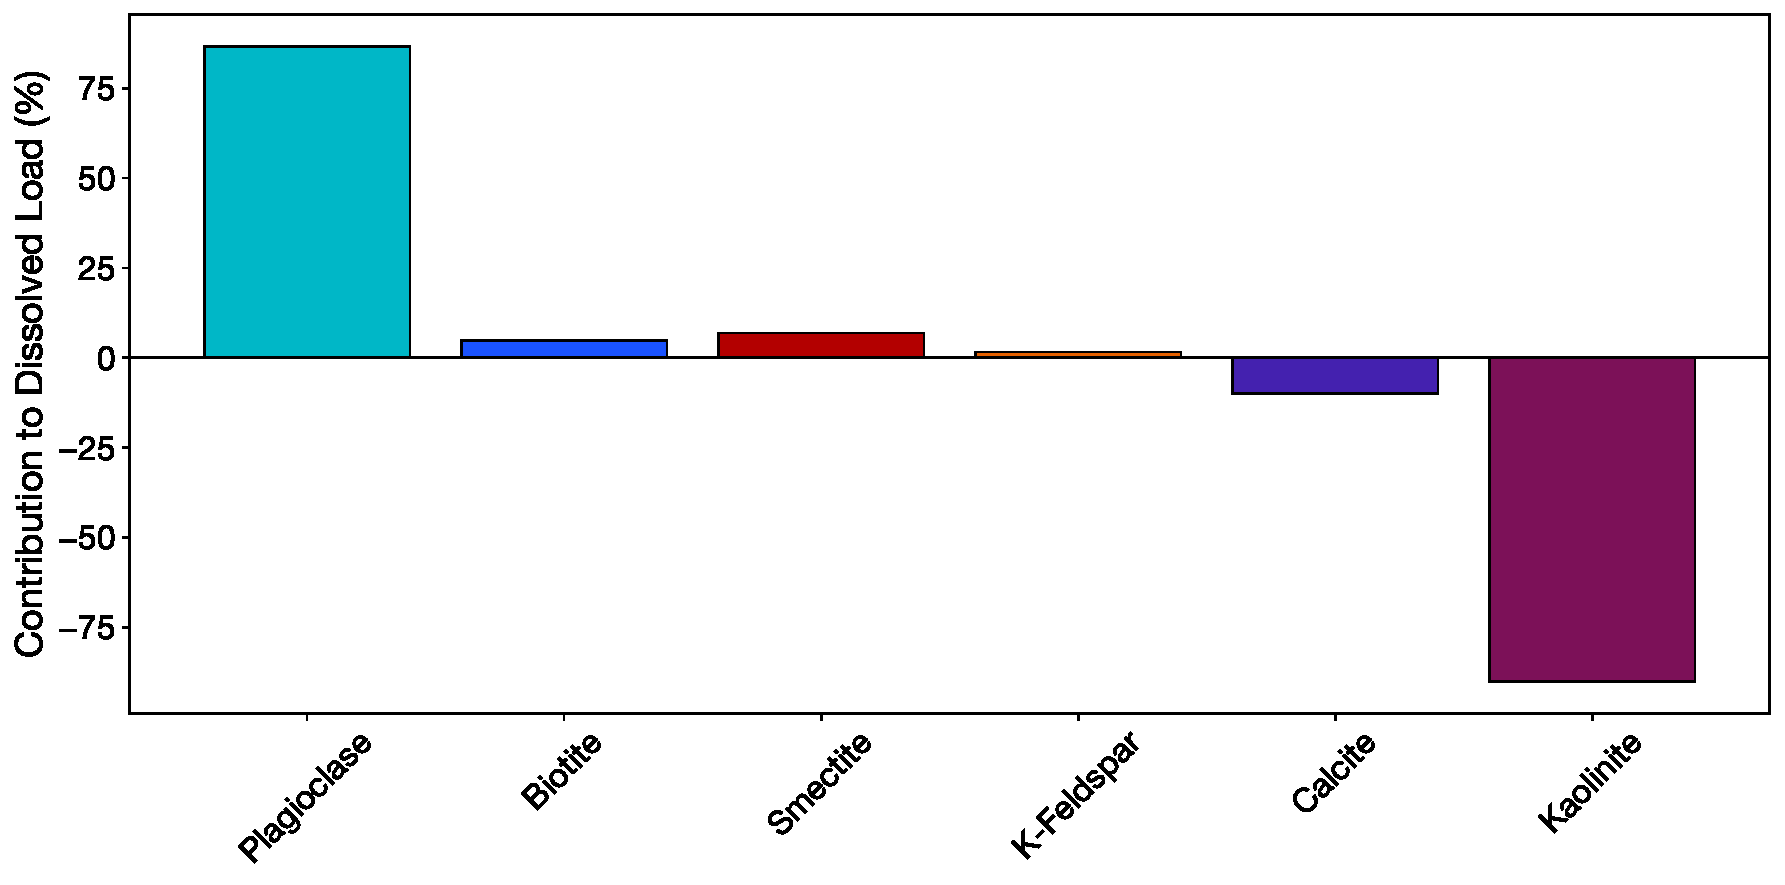
\includegraphics[width=\textwidth]{Normalized_Average_Mineral_Volume_Changes.pdf}
    \caption{Modal Decomposition results averaged over all springs. y-axis corresponds to volumetric proportion of mineral contributing to the dissolved (measured) load. Negative y-space indicates the mineral is involved in the backward reaction.}
    \label{fig:modal}
\end{figure}

\FloatBarrier

Figure \ref{fig:discussion6} is representative of most springs in Traverse 3. Hence, the major phase being dissolved is plagioclase feldspar and the major phase being precipitated is kaolinite. The primary composition of plagioclase in the area corresponds to $\approx$ An-20 (Bickle et al., 2015; Knight et al., 2024).  The plagioclase to kaolinite reaction is given by the following equation (written so that aluminium is conserved):

\begin{equation}
    \begin{matrix}
Ca_{0.20}Na_{0.80}Al_{1.20}Si_{2.80}O_{8} + 1.2H^{+} + 0.6 H_{2}O \\ \rightarrow\\ 0.6 Al_{2}Si_{2}O_{5}(OH)_{4} + 0.8 Na^{+} + 0.2 Ca^{2+} + 1.6 SiO_{2}(aq)
    \end{matrix}
\end{equation}
\quad Or
\begin{equation}
    \begin{matrix}
An_{20} + 1.2 H^{+} + 0.6 H_{2}O\\ \rightarrow\\ 0.6 Kaolinite + 0.8 Na^{+} + 0.2 Ca^{2+} + 1.6 SiO_{2}(aq)
\end{matrix}
\label{eq:10}
\end{equation}\\

\newpage


\subsection{One-Dimensional Reactive Transport Models}

Reactive transport models are widely used in applied fluid dynamics and various fields within Earth Sciences. These models aim to track chemical reactions occurring at each spatial point, accounting for the movement of reactants to and reaction products away from those points (Bethke, 2011). The basic form of a reactive transport model is a partial differential equation that describes the transport of solutes and the reactions that occur between them. For reacting solutes, concentration changes over time are governed by transport rates — derived from the divergence principle — and the relative rates of dissolution and precipitation (Bethke, 2011). These models simplify a real world three-dimensional catchment into one-dimensional flow paths. Additionally, as described in the Introduction ref, porosity is chosen to be a representative average over the whole subsurface; this allows for the results to feasibly represent residence times that come from channelised or slow porous flow. The proposed equations can be complex, but in simple cases a species of concentration $C_i$ can be modelled to follow a first-order rate law, generally represented by:

\begin{equation}
    \frac{\partial C_i}{\partial t} = \mathcal{O}_{T}(C_i) + \mathcal{O}_{R}(C_i)
    \label{eq:1}
\end{equation}\\


Where \(\mathcal{O}_{T}\) and \(\mathcal{O}_{R}\) are the transport and reaction operators, respectively (Bethke, 2011). Depending on the hypothesis supported, equation \ref{eq:1} can be modified accordingly. The following sections will discuss two models with their own versions of equation \ref{eq:1}.

\subsubsection*{Model Motivation}

As discussed in the Introduction (ref), there are different hypotheses regarding the major controls on chemical weathering. This section will contrast one model following the hypothesis that weathering is most sensitive to temperature (Fontorbe et al., 2013), and another model that suggests weathering is more sensitive to the hydrological cycle (Maher, 2011; Maher and Chamberlain, 2014). The benchmark for a model's effectiveness will be how well it can predict residence times compared to previous studies on gas tracers. Assumptions and constraints will be compared and contrasted, and their results used to inform the calculation of rates of reaction and approach to equilibrium in Melamchi. For both models, the element used to benchmark is dissolved silicon. This is because silicon is present in both dissolution and precipitation reactions, so it is applicable to the Maher model which considers both reactions. Furthermore, silicon is what both models were used for in their respective original studies.


\begin{figure}[h]
    \centering
    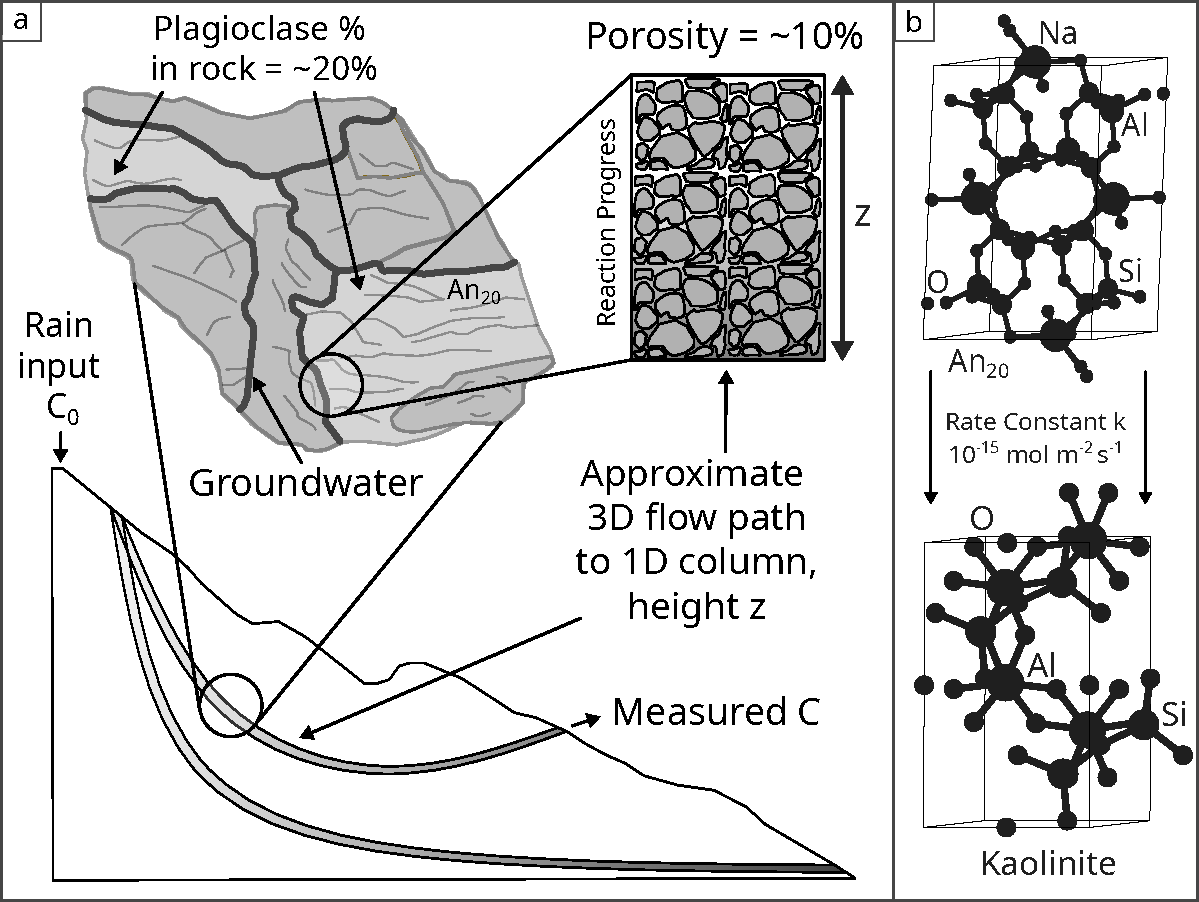
\includegraphics[width=\textwidth]{sketch.pdf}
    \caption{(a) Illustration showing workflow performed in reactive transport models. Sketch shows different parameters used, such as the rain input at the top of the catchment used for the initial "$C_0$" concentration, the plagioclase percentage in the rock as well as the porosity. (b) Mineral ball and spoke models showing the dissolution of plagioclase and precipitation of kaolinite. Ball and Spoke models from CSD (ref)}
    \label{fig:reactsketch}
\end{figure}

\FloatBarrier

\newpage

\subsubsection*{Fontorbe et al. (2013) - Model}

This model investigates silicon isotopic composition in the Ganges River, assuming constant reaction rates along flow paths (see Appendix for a full derivation, and Table ref for a list of parameters used). This model was initially constructed to reproduce DSi concentration and $\delta^{30}$Si in the Ganges, but is being repurposed in a novel fashion for this study. The first-order differential equation governing transport and reaction is given as:\\

    \begin{equation}
    \phi \frac{\partial C}{\partial t} = -\omega \phi \frac{\partial C}{\partial z} + R_n(1-f)
    \end{equation}\\

Where C is the elemental concentration, $\omega$ is the fluid velocity, $\phi$ is the rock porosity, z is a position along the flow path, R$_\text{n}$ is the rate of reaction, and f is the fraction of Si present in the dissolved load that is reprecipitated in the back reaction. The equation can be nondimensionalised using the Damköhler number (\(N_D\)), which describes the relative importance of kinetic vs transport-controlled settings (Bethke, 2008):\\

\begin{equation}
    N_D = \frac{R_n h}{\phi C_0 \omega}
\end{equation}\\

Assuming steady-state (\(\partial C/\partial t = 0\)), the concentration at the end of the flow path can be rearranged to give the residence time \(T_f\):\\

\begin{equation}
    T_f = \frac{(C - C_0)\phi}{(1-f)R_n}
\end{equation}


\begin{table}[H]
    \centering
    \renewcommand{\arraystretch}{1.3} % Adjust row height
    \begin{tabular}{|c|c|c|c|}
        \hline
        \multicolumn{4}{|c|}{\textbf{Fontorbe}} \\  
        \hline
        \textbf{Parameter} & \textbf{Definition} & \textbf{Units} & \textbf{Formula (Value)} \\  
        \hline
        $\phi$ & Porosity & - & 0.1 $^*$\\
        $\omega$ & Fluid velocity & m/s & Variable \\
        $h$ & Length of flow path & m & Variable \\
        $C$ & Concentration \@ end of flow path & $\mu$mol/L & Variable \\
        $C_0$ & Initial concentration & $\mu$mol/L & Rain Input \\
        $f$ & Fraction reprecipitated & - & 0.5$^*$ \\
        $N_D$ & Damkohler Number & - & $N_D = \frac{R_n h}{\phi C_0 \omega}$ \\
        $T_f$ & Residence time & s & $T_f = \frac{h}{\omega\phi}$ \\
        $R_n$ & Reaction rate & mol/m$^3$/s & $\rho \cdot 10^6 \cdot k \cdot S \cdot X $ \\
        $k$ & Dissolution rate constant & mol/m$^2$/s & 10$^{-15*}$ \\
        $S$ & Specific surface area & m$^2$/g & 0.1$^*$ \\
        $\rho$ & Plagioclase density & g/cm$^3$ & 2.7$^*$ \\
        $X$ & Volume fraction of mineral in rock & $g_{min}/g_{rock}$ & 0.2$^*$ \\
        \hline
    \end{tabular}
    \caption{Key parameters and definitions for the Fontorbe model. Starred terms are values used for calculation.}
    \label{tab:fontorbe1}
\end{table}


\FloatBarrier









\newpage




\subsubsection*{Maher and Chamberlain (2014) Model}

This model is built in accordance with the principle that the main control on silicate weathering is hydrological cycle, namely how much water passes flows a particular path. The model is based on the assumption that the reaction rate decreases linearly with approach to equilibrium, and that all weathering paths approach equilibrium. The motivation behind the hydrological control is based on sensitivity analyses of real catchment data on one-dimensional reactive transport models which suggest that porosity, mineral surface area, and temperature have no consistent correlation with water composition (Maher, 2011). See Appendix and Table ref for a full derivation and the model parameters respectively. The model begins with the following representation of the concentration of a solute in a fluid flow path:\\ 

\begin{equation}
    \frac{dC}{dt} = -\frac{q}{\theta} \frac{dC}{dz} + \sum_i \mu_i R_{d,i} \left( 1 - \left( \frac{C}{C_{eq}} \right)^{n_i} \right)^{m_i} - \sum_i \mu_i R_{p,i} \left( 1 - \left( \frac{C}{C_{eq}} \right)^{n_i} \right)^{m_i}
\end{equation}

Where \( C \) is the concentration, \( q \) is the fluid flux, \( \theta \) is the volumetric water content, \( z \) is the position along the flow path, \( \mu \) is the stoichiometric coefficient, \( R \) is the rate of reaction for dissolution and precipitation respectively, \( C_{eq} \) is the equilibrium concentration, and \( n \) and \( m \) are non-linear parameters (Maher and Chamberlain, 2013). For a given packet of water, R$_{\text{n}}$ is defined as: \\

\begin{equation}
R_n = R_{d} - R_{p}
\end{equation} 
\begin{equation}
\frac{dc}{dt} = R_n \left( 1 - \frac{C}{C_{\text{eq}}} \right)
\end{equation} \\

Where R$_d$ and R$_p$ are the rates of dissolution and precipitation respectively. This can be solved for concentration, and rearranged for residence time to obtain:\\

\begin{equation}
    T_f = \frac{C_{eq} \cdot \left(C - C_0\right)}{e^2 R_n \left( C_{\text{eq}} - C \right)}
\end{equation}\\

Note the $e^2$ term is used because the Maher model considers all paths as if they approach equilibrium.

\begin{table}[H]
    \centering
    \renewcommand{\arraystretch}{1.3} % Adjust row height
    \begin{tabular}{|c|c|c|c|}
        \hline  % DOUBLE BOLD LINE
        \multicolumn{4}{|c|}{\textbf{Maher}} \\  
        \hline
        \textbf{Parameter} & \textbf{Definition} & \textbf{Units} & \textbf{Formula (Value)} \\
        \hline
        $\phi$ & Porosity & - & 0.1$^*$ \\
        $h$ & Length of flow path & m & Variable \\
        $q$ & Flow rate & m/s & Variable \\
        $C_{eq}$ & Equilibrium concentration & $\mu$mol/L & Max Catchment \\
        $C_0$ & Initial concentration & $\mu$mol/L & Rain Input \\
        $R_n$ & Net reaction rate & mol/L/s & $\rho \cdot 10^6 \cdot k \cdot S \cdot X $ \\
        $\rho$ & Plagioclase density & g/cm$^3$ & 2.7$^*$ \\
        $k$ & Dissolution rate constant & mol/m$^2$/s & 10$^{-15*}$ \\
        $S$ & Specific surface area & m$^2$/g & 0.1$^*$ \\
        $X$ & Volume fraction of mineral in rock & $g_{min}/g_{rock}$& 0.2$^*$ \\
        $\tau$ & Scaling factor & - & $\tau = e^2$ \\
        $D_w$ & Damkohler Coefficient & m$^2$/s & $D_w = \frac{L \phi R_n}{C_{\text{eq}}}$ \\
        $T_f$ & Residence time & s & $T_f = \frac{h \phi}{q}$ \\
        \hline
    \end{tabular}
    \caption{Key parameters and definitions for the Maher model. Starred terms are values used for calculation.}
    \label{tab:maher1}
\end{table}

\FloatBarrier


\subsection{Estimates of Uncertainty}

Uncertainties were propagated using a Monte Carlo method using an assumed normal distribution and 1000 simulations. Both the observed parameters and estimated parameters have uncertainties associated to them.


\begin{table}[H]
    \centering
    \renewcommand{\arraystretch}{1.3} % Adjust row height
    {\small
    \begin{tabular}{|c|c|c|c|c|}
        \hline
        \multicolumn{5}{|c|}{\textbf{Parameter Definitions and Propagated Uncertainties}} \\  
        \hline
        \textbf{Parameter} & \textbf{Definition} & \textbf{Units} & \textbf{Value} & \textbf{Uncertainty} \\  
        \hline
        $\phi$ & Porosity & - & 0.1 & $\pm$ 10\% \\  
        $C_{eq}$ & Equilibrium DSi concentration & $\mu$mol/L & 869 $\mu$mol/L & $\pm$ 10\% \\  
        $C_0$ & Initial DSi concentration & $\mu$mol/L & 95 $\mu$mol/L & $\pm$ 10\% \\  
        $\rho$ & Plagioclase density & g/cm$^3$ & 2.7 & $\pm$ 10\% \\  
        $k$ & Dissolution rate constant & mol/m$^2$/s & 10$^{-15}$ & $\pm$ 10\% \\  
        $S$ & Specific surface area & m$^2$/g & 0.1 & $\pm$ 10\% \\  
        $X$ & Volume fraction of mineral in rock & $\text{g}_{\text{min}}/\text{g}_{\text{rock}}$ & 0.2 & $\pm$ 10\% \\   
        $f$ & Fraction reprecipitated & - & 0.5 & $\pm$ 10\% \\
        $\Delta G^0$ & Standard Gibbs Free Energy & kJ/mol & $\text{-RTlnK}^*$ & $\pm$ 10\% \\
        \hline
    \end{tabular}}
    \caption{Key parameters, definitions, and propagated uncertainties. $^*$: Uncertainty associated with temperature and K calculated from pgcc using The Geochemist's Workbench® Rxn program(ref)}
    \label{tab:montecarlo}
\end{table}

\FloatBarrier




% This leverages randomness to calculate uncertainties. Both observed and estimated parameters have uncertainties associated with them. Each Monte Carlo simulation randomly varies the input parameters within their estimated uncertainty ranges. Once many simulations have been run, the distribution of results reflects the possible range of values obtained for a given relationship. The uncertainty is then calculated as two standard deviations of the mean of the distribution.


\newpage




\section{Results: Differences in Spring Chemistry and Residence Time}

\subsection{Traverse 1}

\begin{figure}[h]
    \centering
        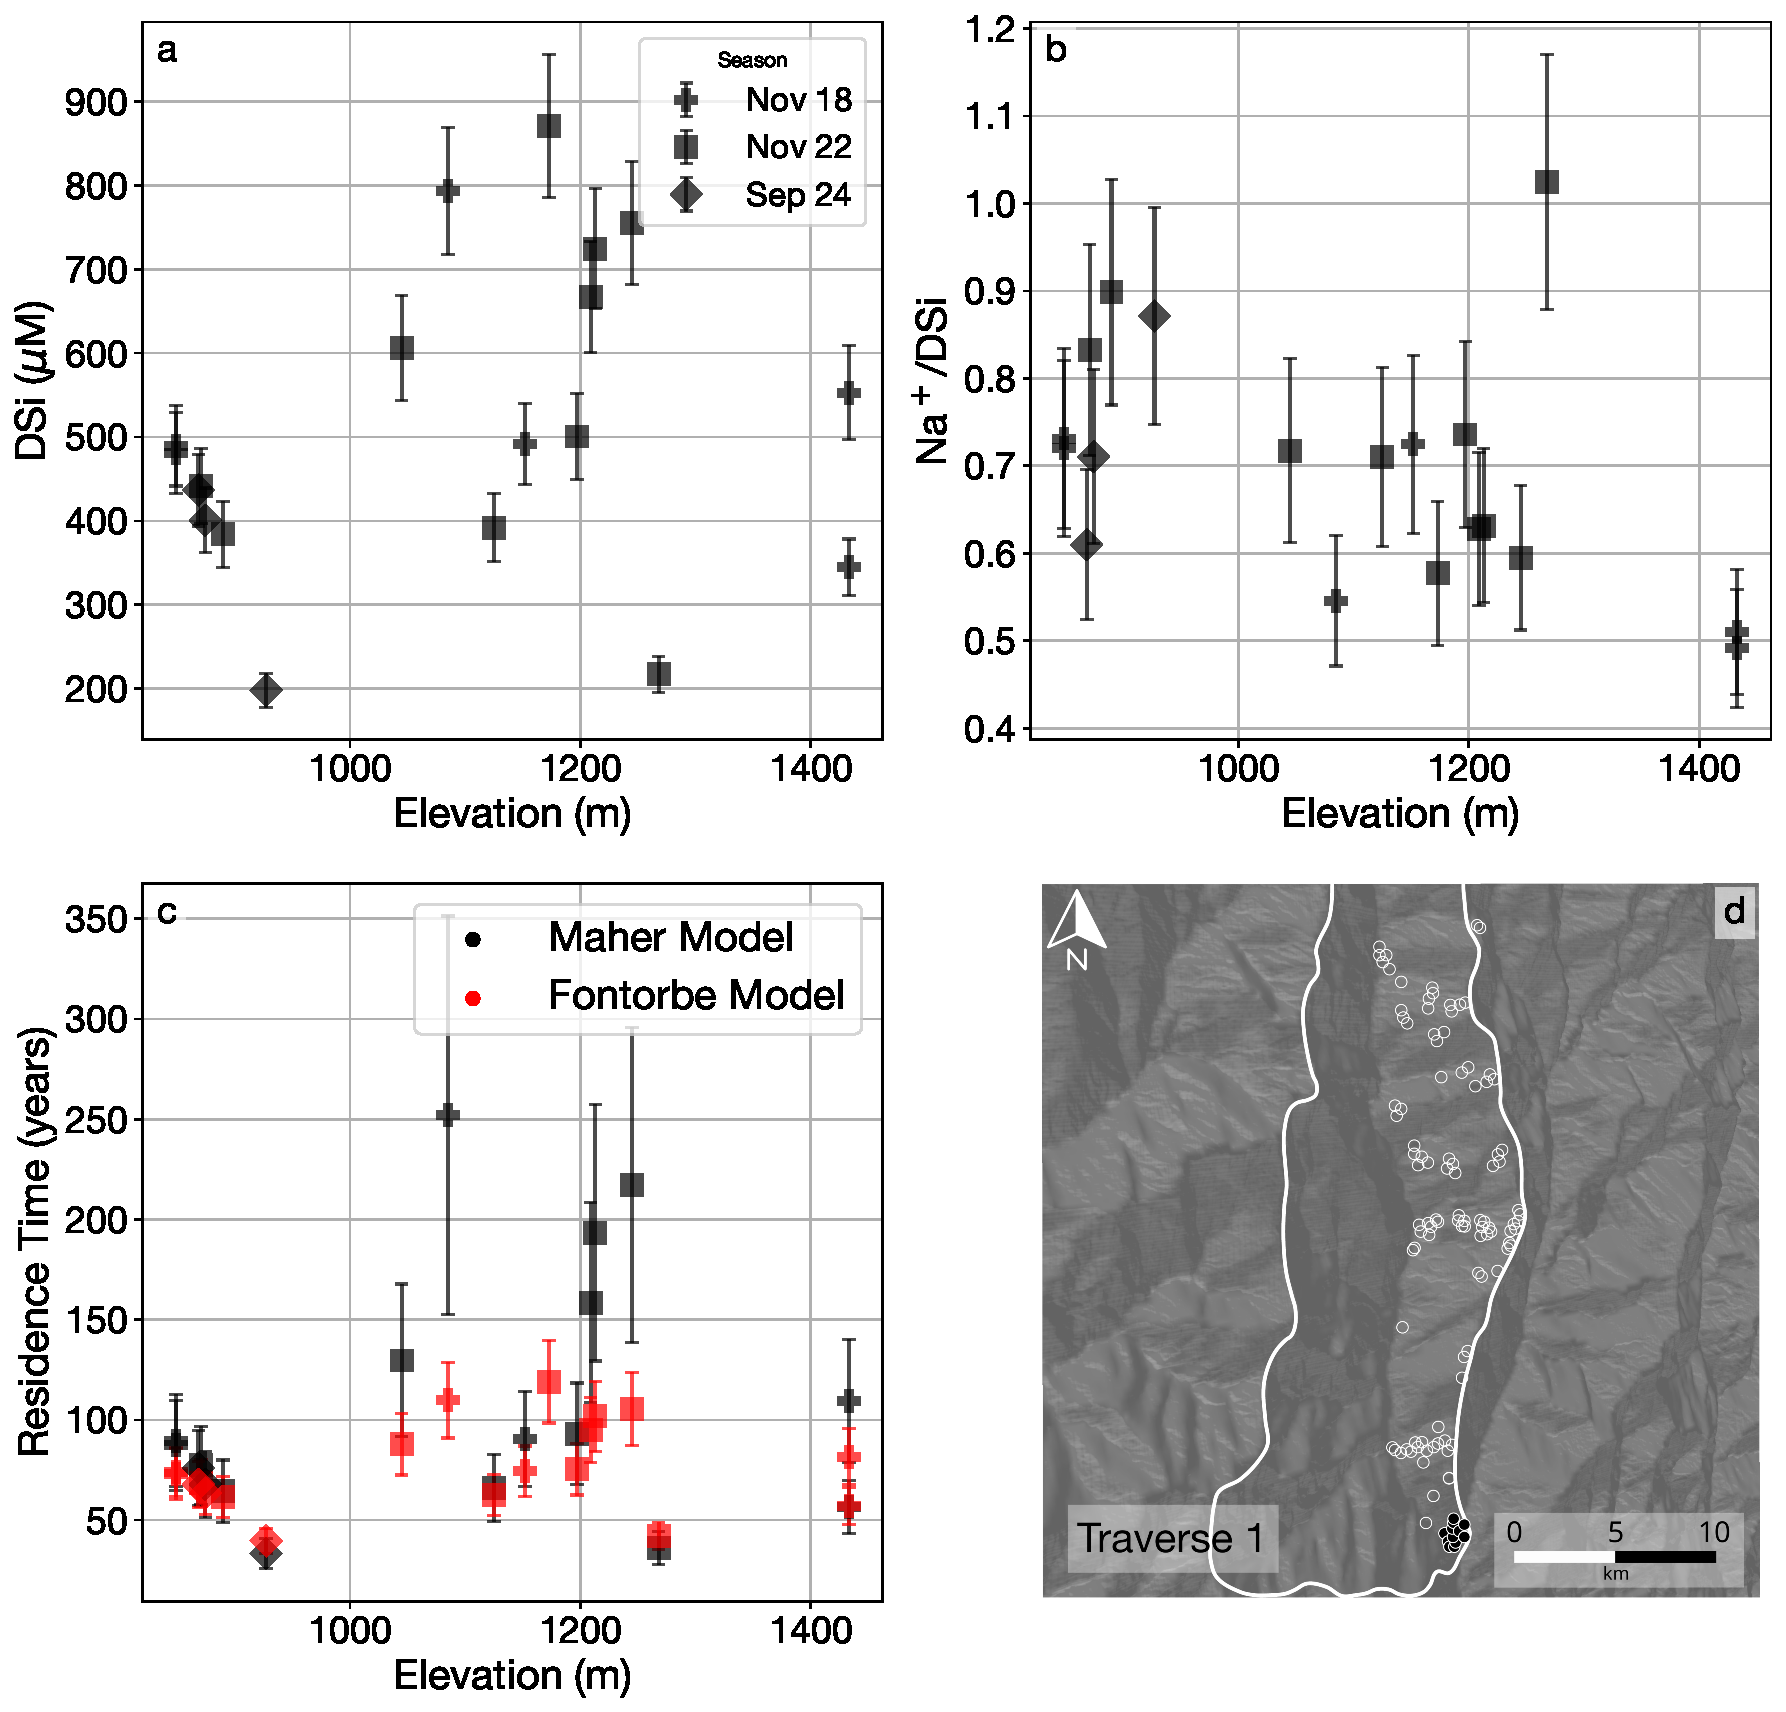
\includegraphics[width=\textwidth]{Traverse_1_summary.pdf}
    \caption{Traverse 1 - Variations in Spatial Chemistry}
    \label{fig:spatial_changes_spring1}
\end{figure}

\FloatBarrier

Concentration of dissolved silicon (DSi) in the springs sampled in Traverse 1 is at a maximum for the whole catchment. There is no clear trend of increasing DSi concentration with decreasing elevation, but Na/Si does increase with the same x-axis. The Fontorbe model predicts a peak of $\approx$ 100 years, while the Maher model predicts a much higher residence time of $\approx$ 600 years. 


% Strontium isotopes are also at a maximum in this traverse, but there is no resolvable mixing trend; strontium isotope ratios used alongside strontium concentrations can be used to determine mixing between different endmembers (Faure, 1986; See Appendix).



\newpage

\subsection{Traverse 2}

\begin{figure}[h]
    \centering
        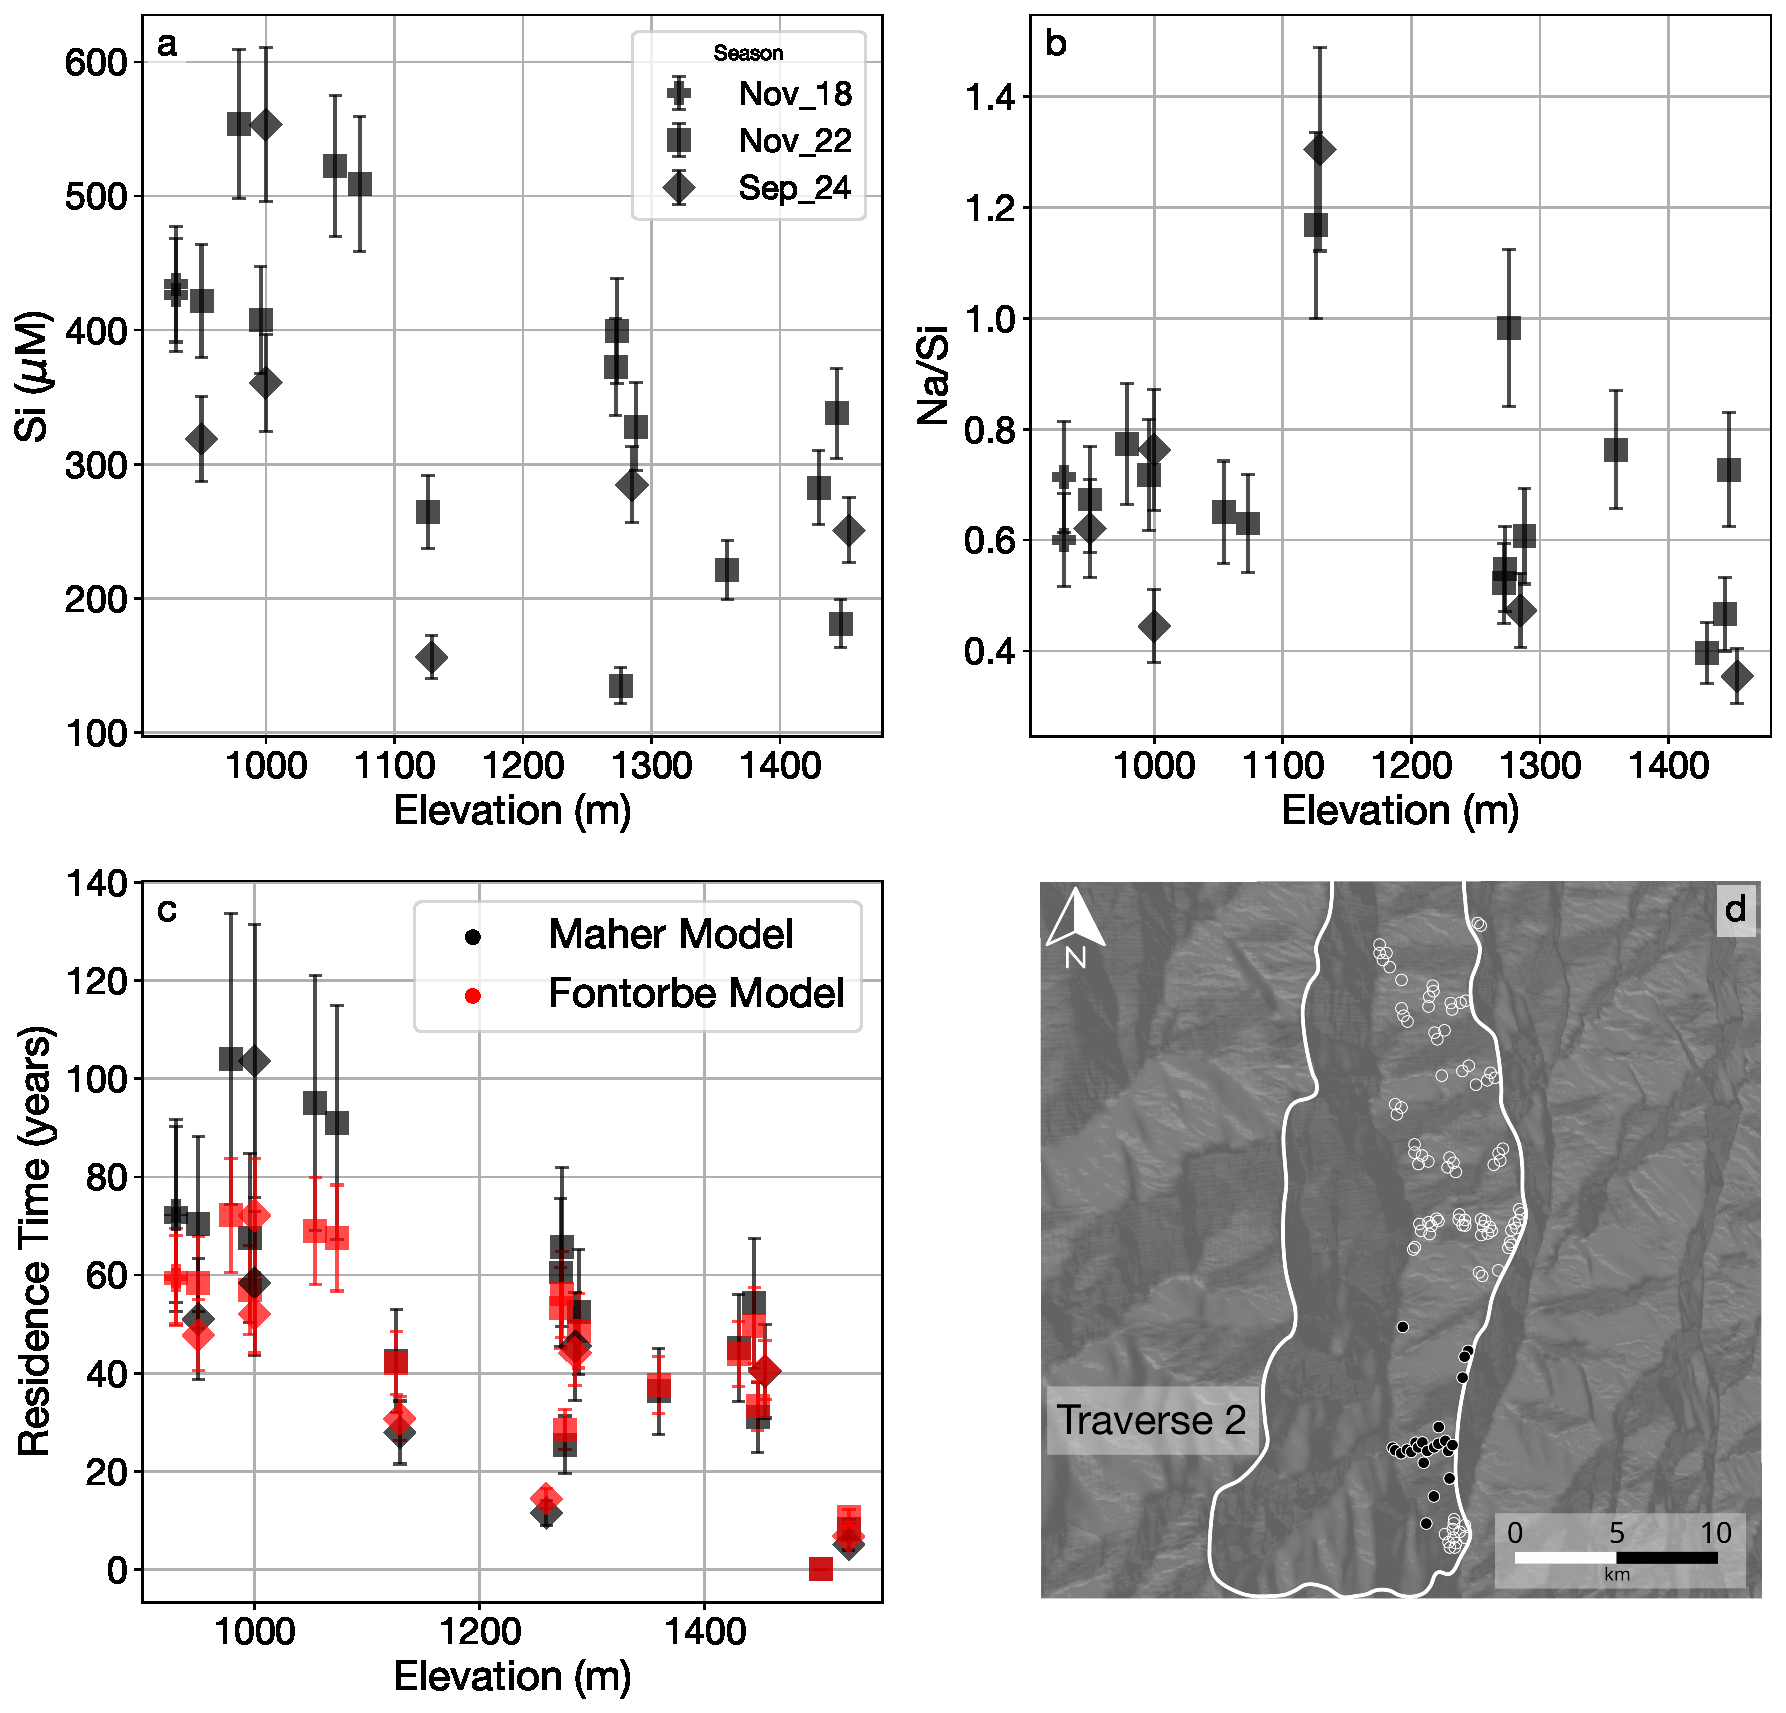
\includegraphics[width=\textwidth]{Traverse_2_summary.pdf}
    \caption{Traverse 2 - Variations in Spatial Chemistry}
    \label{fig:spatial_changes_spring2}
\end{figure}

\FloatBarrier

Dissolved silicon concentration shows a clear increase in concentration with decreasing elevation. There is no resolvable trend with Na/Si and elevation, nor with different seasons when it was collected. Residence times are generally lower than those in Traverse 1, but the Maher model is still higher at lower elevations, predicting a maximum of $\approx$ 100 years. The Fontorbe model predicts generally older times than the Maher model at higher elevations, and lower times at lower elevations. 


% Strontium isotopes are in the same range as those in Traverse 1. Here, a mixing trend is resolvable given by a straight line with a R$^2$ of (?).
% The lack of trend in Na/Si against elevation space, coupled with the consistent increase in DSi suggests little reprecipitation is occuring in this traverse. The lower residence times compared to Traverse 1 are consistent with shorter flow paths at higher elevation, considering rainfall which acts as an input to the system is delivered mostly to the top quarter of the catchment, which Traverse 2 is not in. Mixing trends in strontium isotopes suggest a varying lithology that the springs travel through.



\newpage

\subsection{Traverse 3}

\begin{figure}[h]
    \centering
        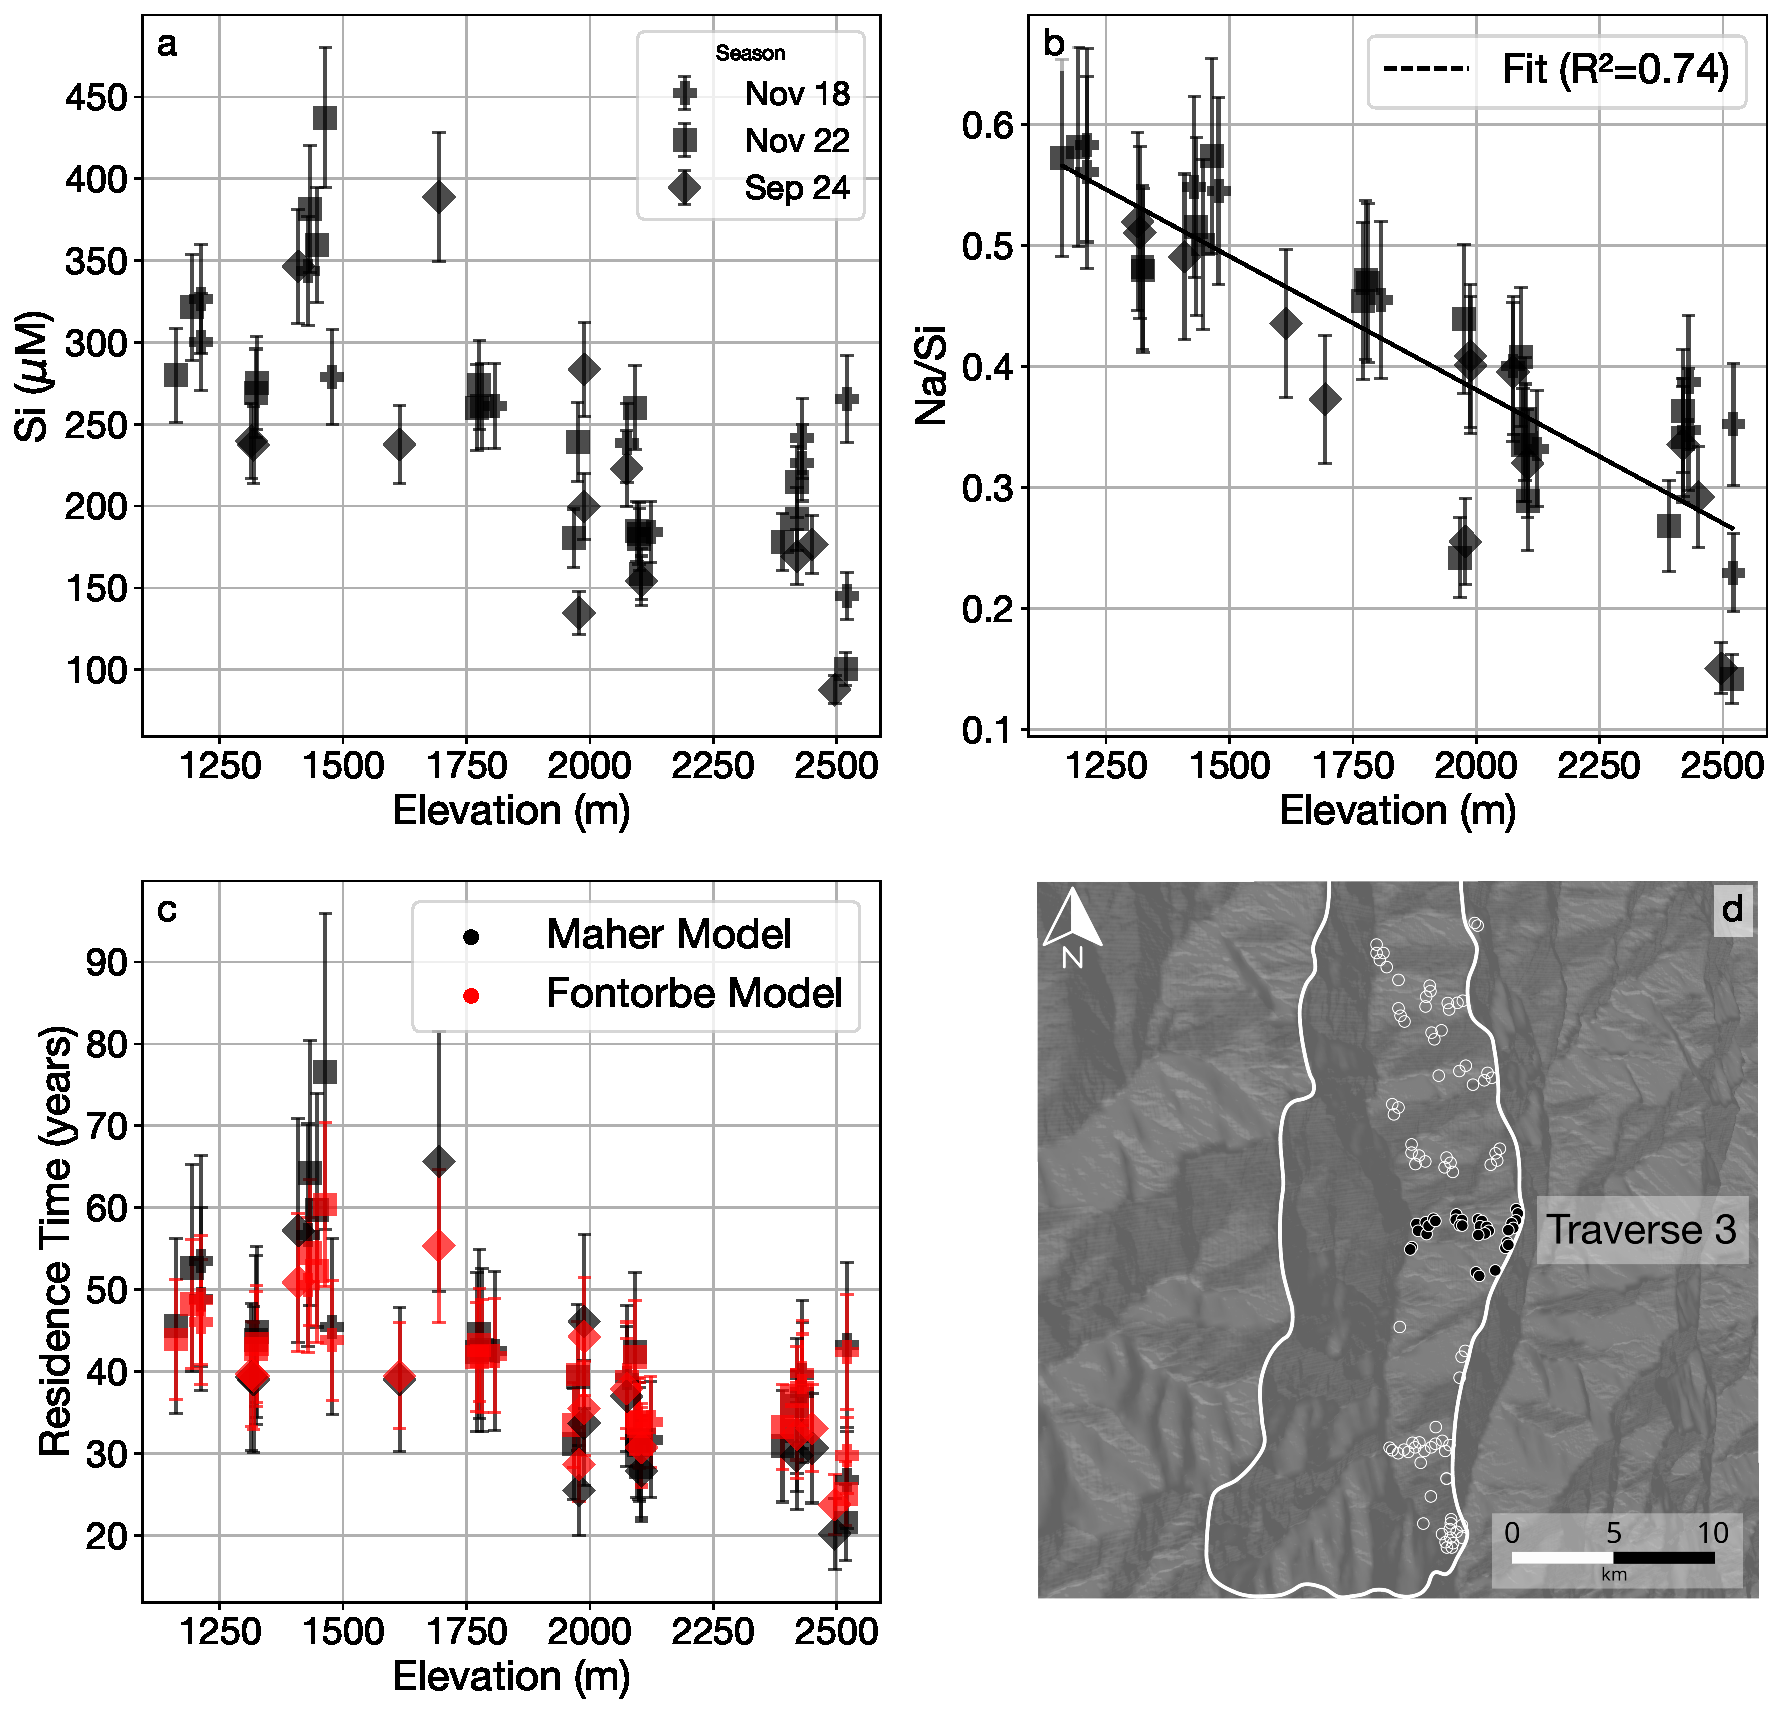
\includegraphics[width=\textwidth]{Traverse_3_summary.pdf}
    \caption{Traverse 3 - Variations in Spatial Chemistry}
    \label{fig:spatial_changes_spring3}
\end{figure}

\FloatBarrier

Dissolved silicon concentration increases with decreasing elevation in Traverse 3. There is a potential dip at the lowermost elevation sampled. Na/Si showcases a consistent increase with decreasing elevation, and this trend carries through between different seasons. Residence times predicted increase as elevation decreases, peaking at $\approx$ 50 years for the Maher model. At the very end of the flow path, however, both the Maher and Fontorbe model predict $\approx$ 25 years. 

%Strontium isotopes do not showcase a clear mixing trend, and the radiogenic strontium isotope values are lower than those found in Traverse 1 and 2. 


\newpage

\subsection{Traverse 4}

\begin{figure}[h]
    \centering
        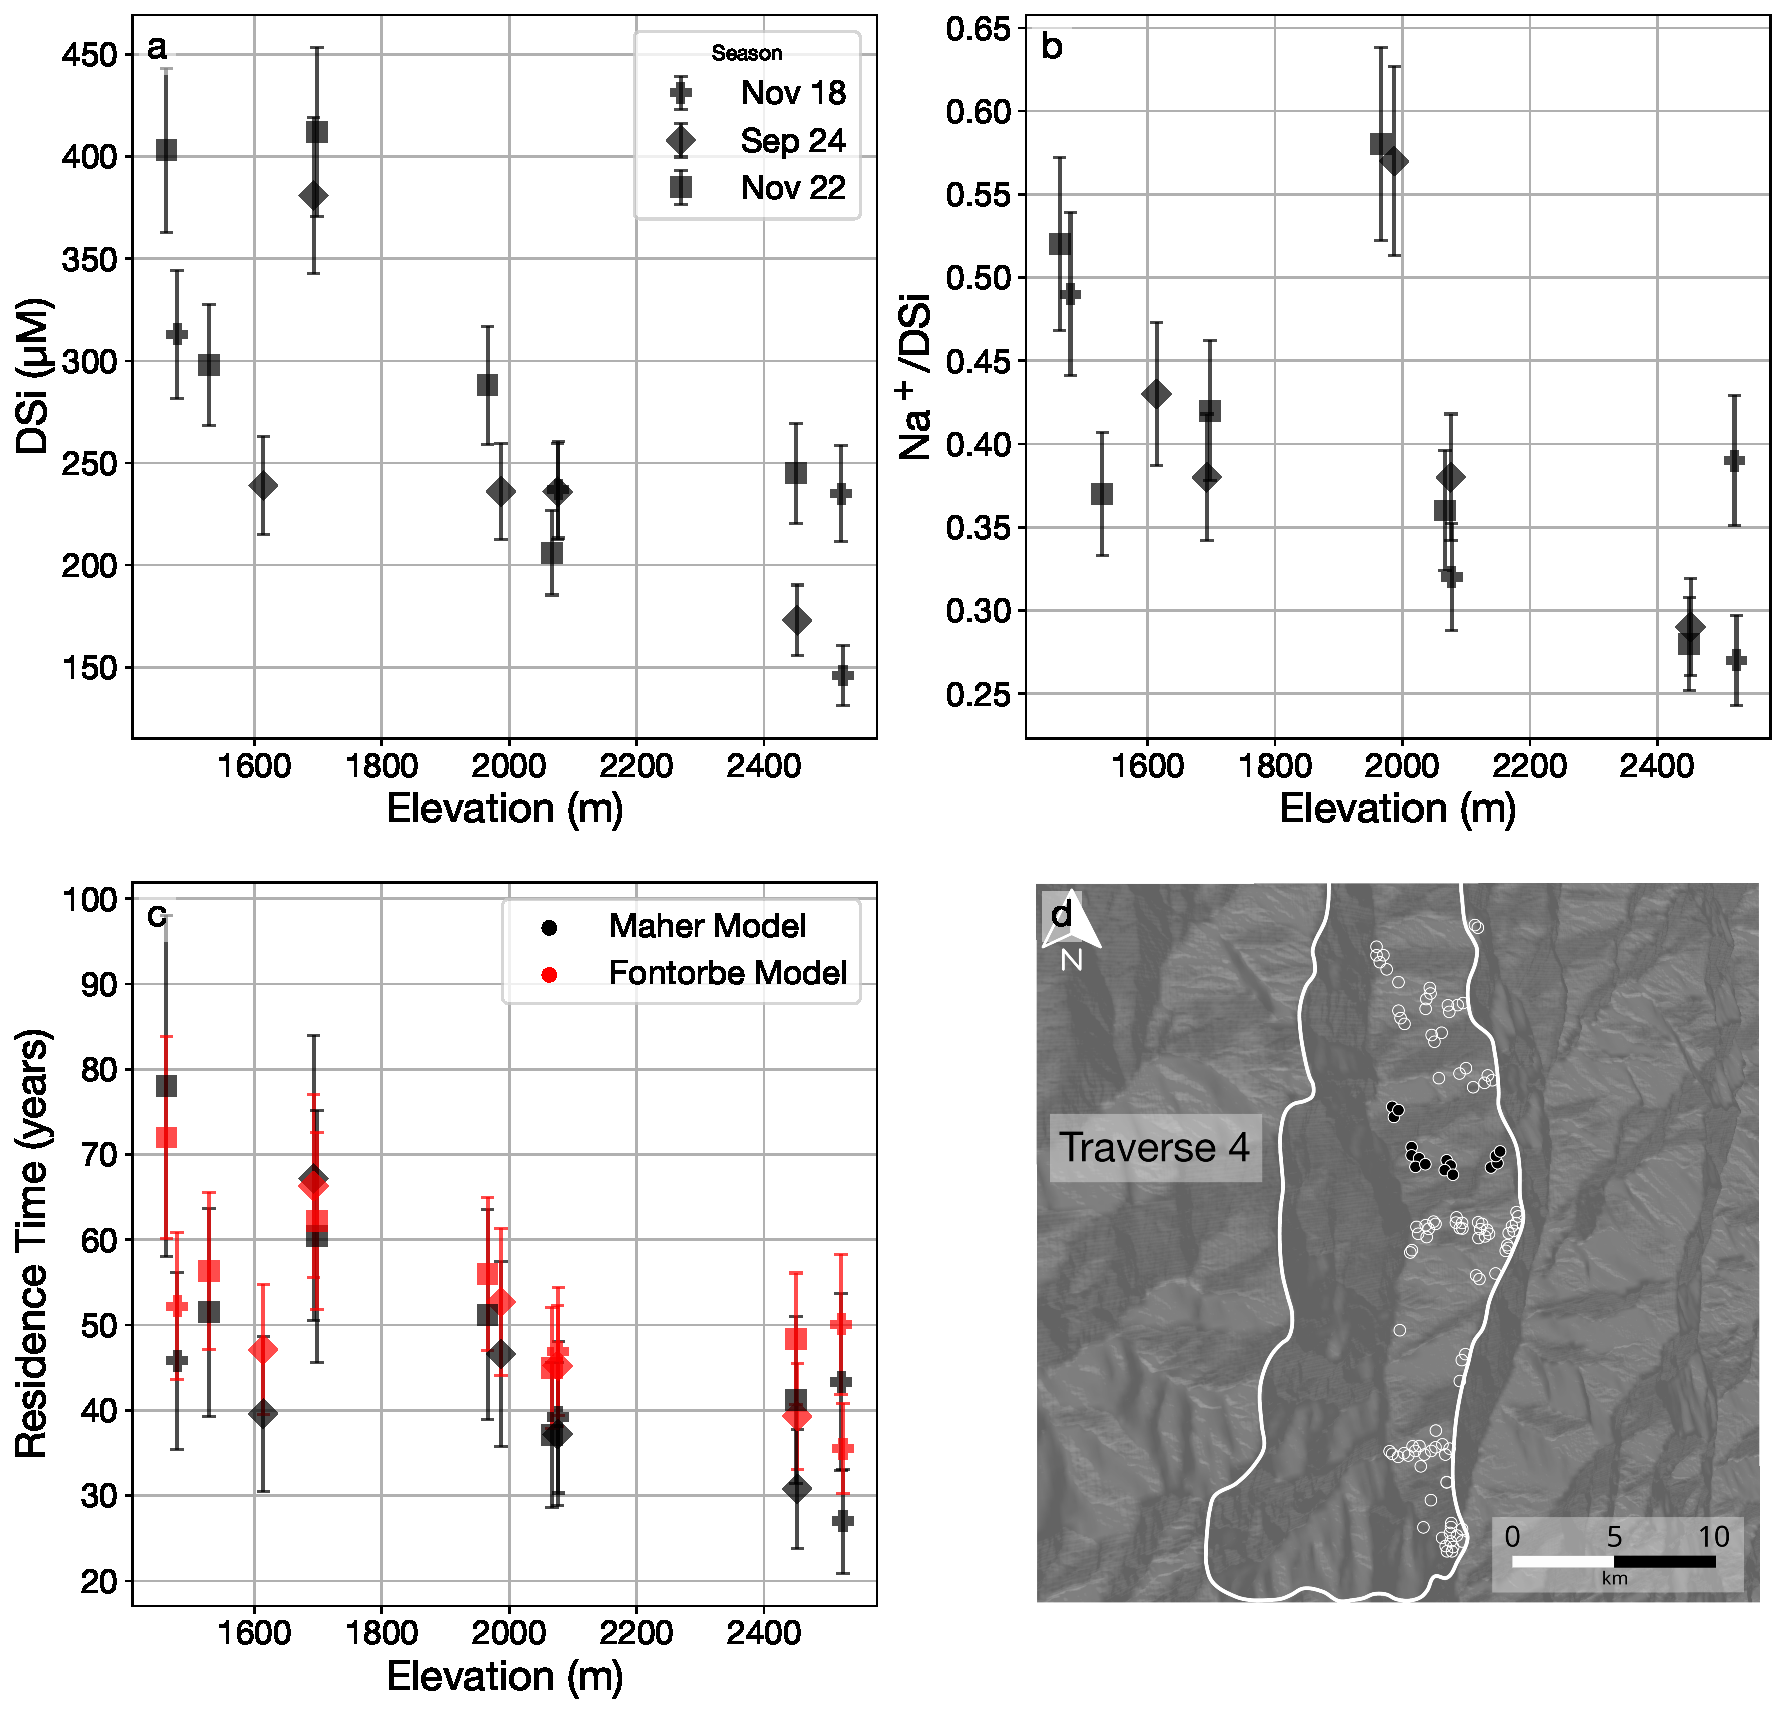
\includegraphics[width=\textwidth]{Traverse_4_summary.pdf}
    \caption{Traverse 4 - Variations in Spatial Chemistry}
    \label{fig:spatial_changes_spring4}
\end{figure}

\FloatBarrier

Traverse 4 is undersampled compared to the other traverses. Given the small sample set, any apparent trend is less to be reflective of the true chemistry. Nevertheless, DSi increases with decreasing elevation as seen in some of the previous traverses. There is no discernable trend with Na/Si. Residence times also increase with decreasing elevation, with the Maher model predicting younger times at the highest elevations, and older times at the lowest elevations. The highest residence times predicted are $\approx$ 35 years.

%Strontium isotopes do not show a clear mixing trend, but the minimum signature is lower than that of Traverse 3.

\newpage

\subsection{Traverse 5}

\begin{figure}[h]
    \centering
        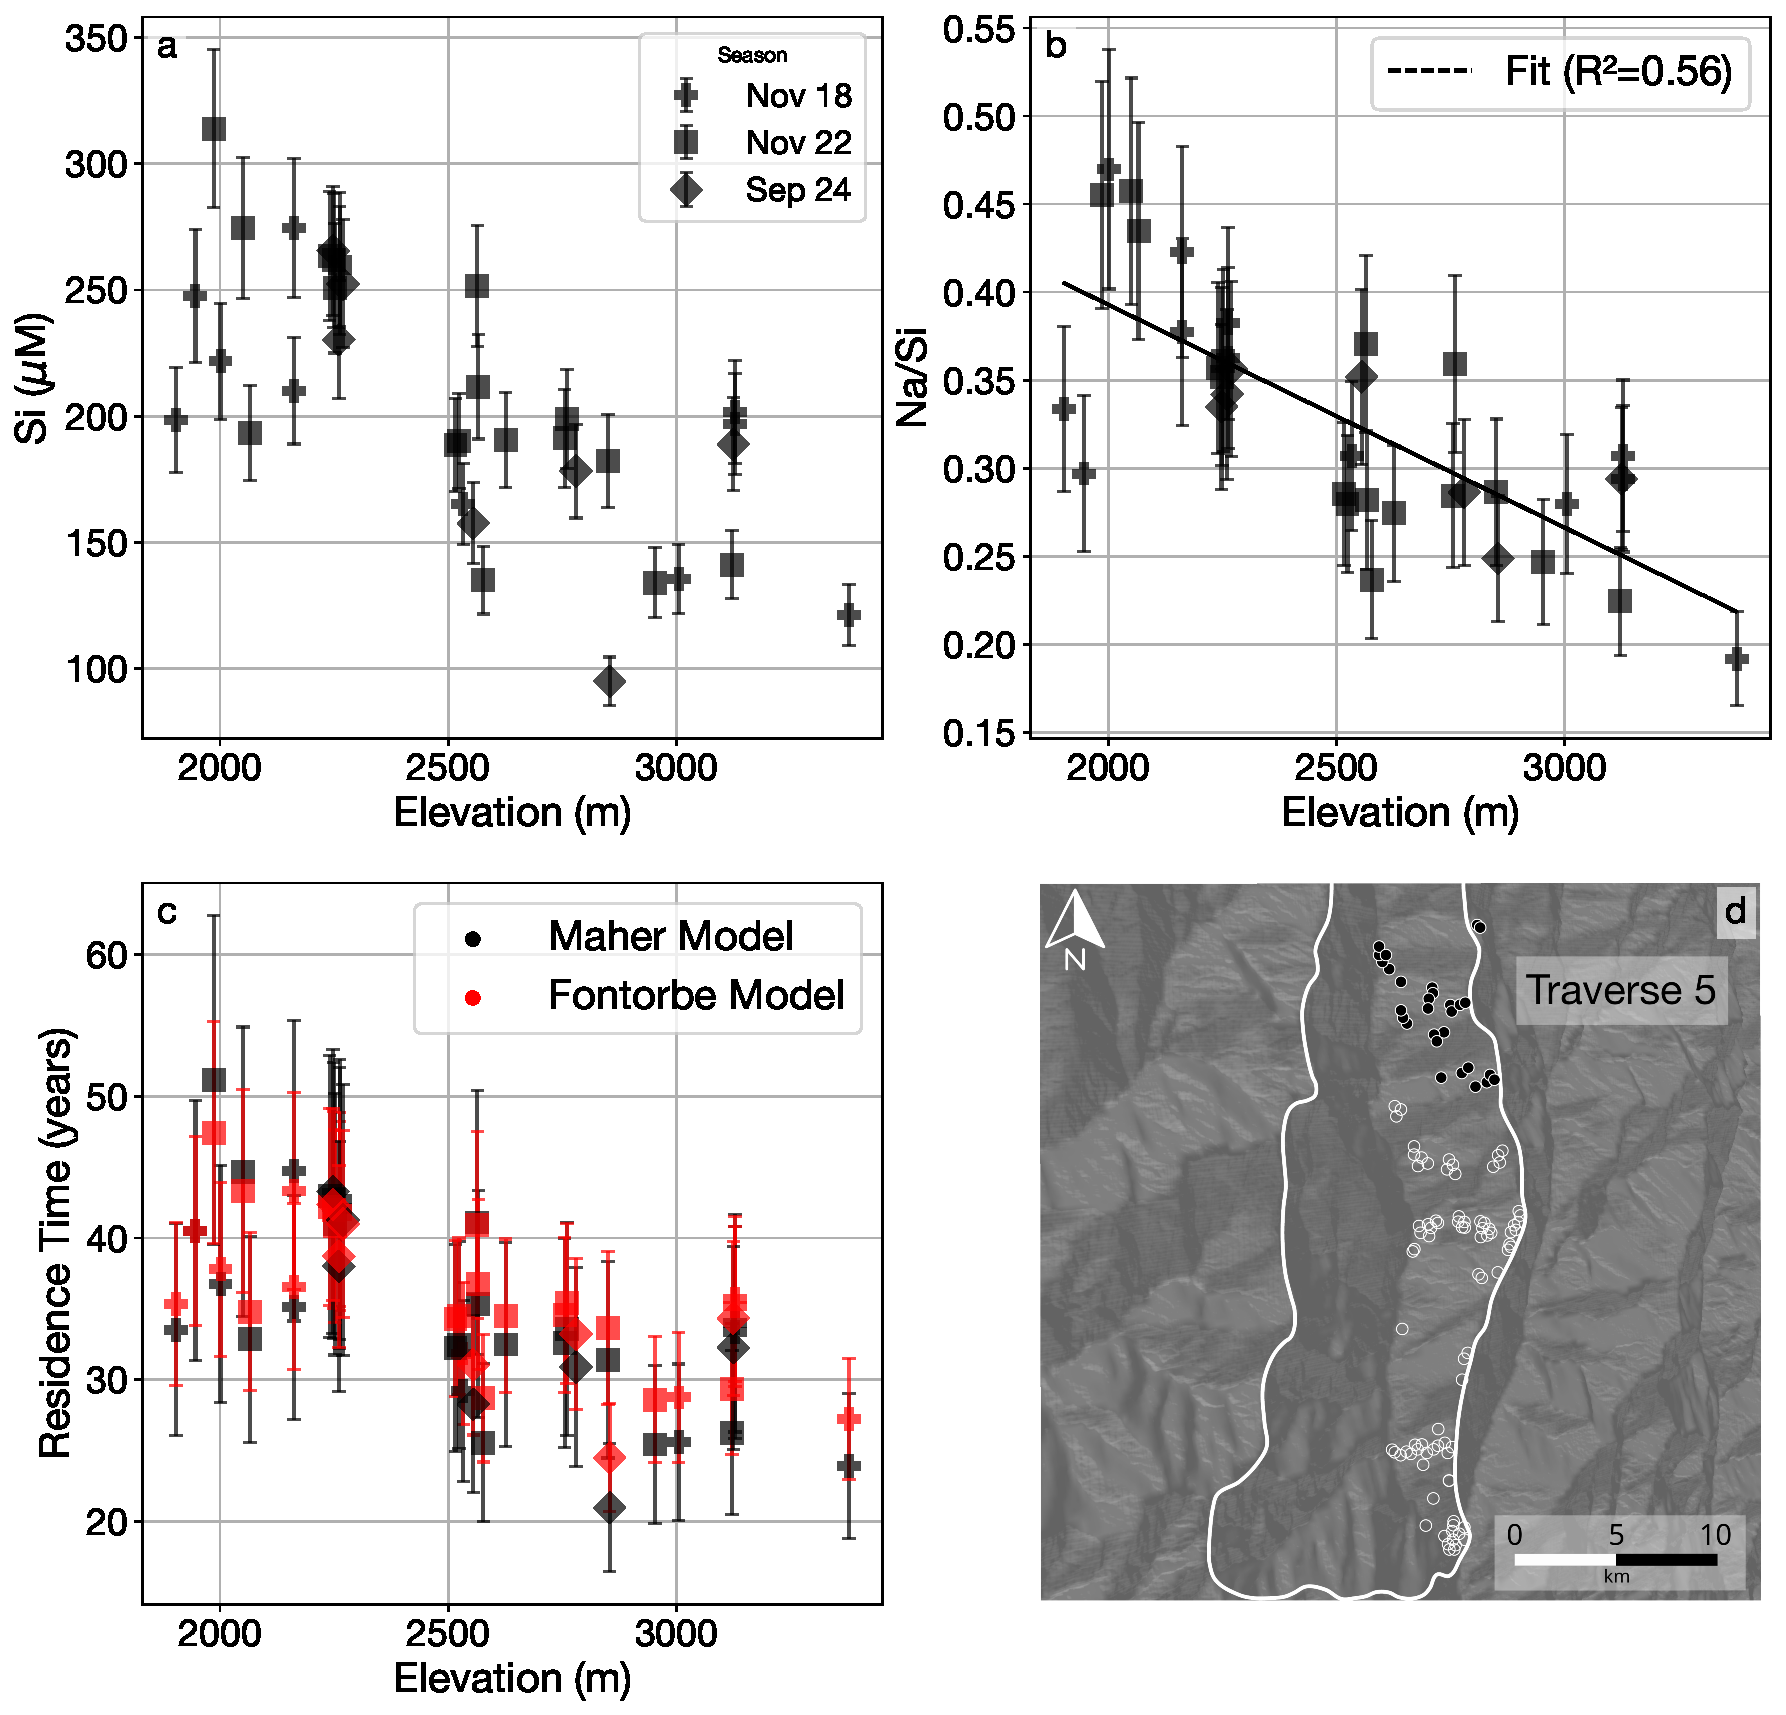
\includegraphics[width=\textwidth]{Traverse_5_summary.pdf}
    \caption{Traverse 5 - Variations in Spatial Chemistry}
    \label{fig:spatial_changes_spring5}
\end{figure}

\FloatBarrier

Traverse 5 is highly sampled and sits at the highest elevation of the whole catchment. DSi concentration increases with decreasing elevation but there is noticeable scatter in the data. Na/Si similarly shows a trend of increasing ratio with decreasing elevation, and it is replicated between different seasons, with considerable scatter. Residence times are the lowest predicted in the catchments.

%, and so are the strontium isotope values.


\subsection{Time Series Trends}

Concentrations of dissolved silicon in several springs in the catchment show a consistent decrease in concentration with the onset of the monsoon. Concentrations are high in April, decrease to a minimum in September, then slowly increase back to April levels through October and November. Decrease in concentration is likely a sign of dilution from increased precipitation during the monsoon. Such a trend is also present in a time series of a spring in Traverse 3. The average April-September decrease is small compared to the average dissolved silicon concentration of the rain.


\begin{figure}[h]
    \centering
    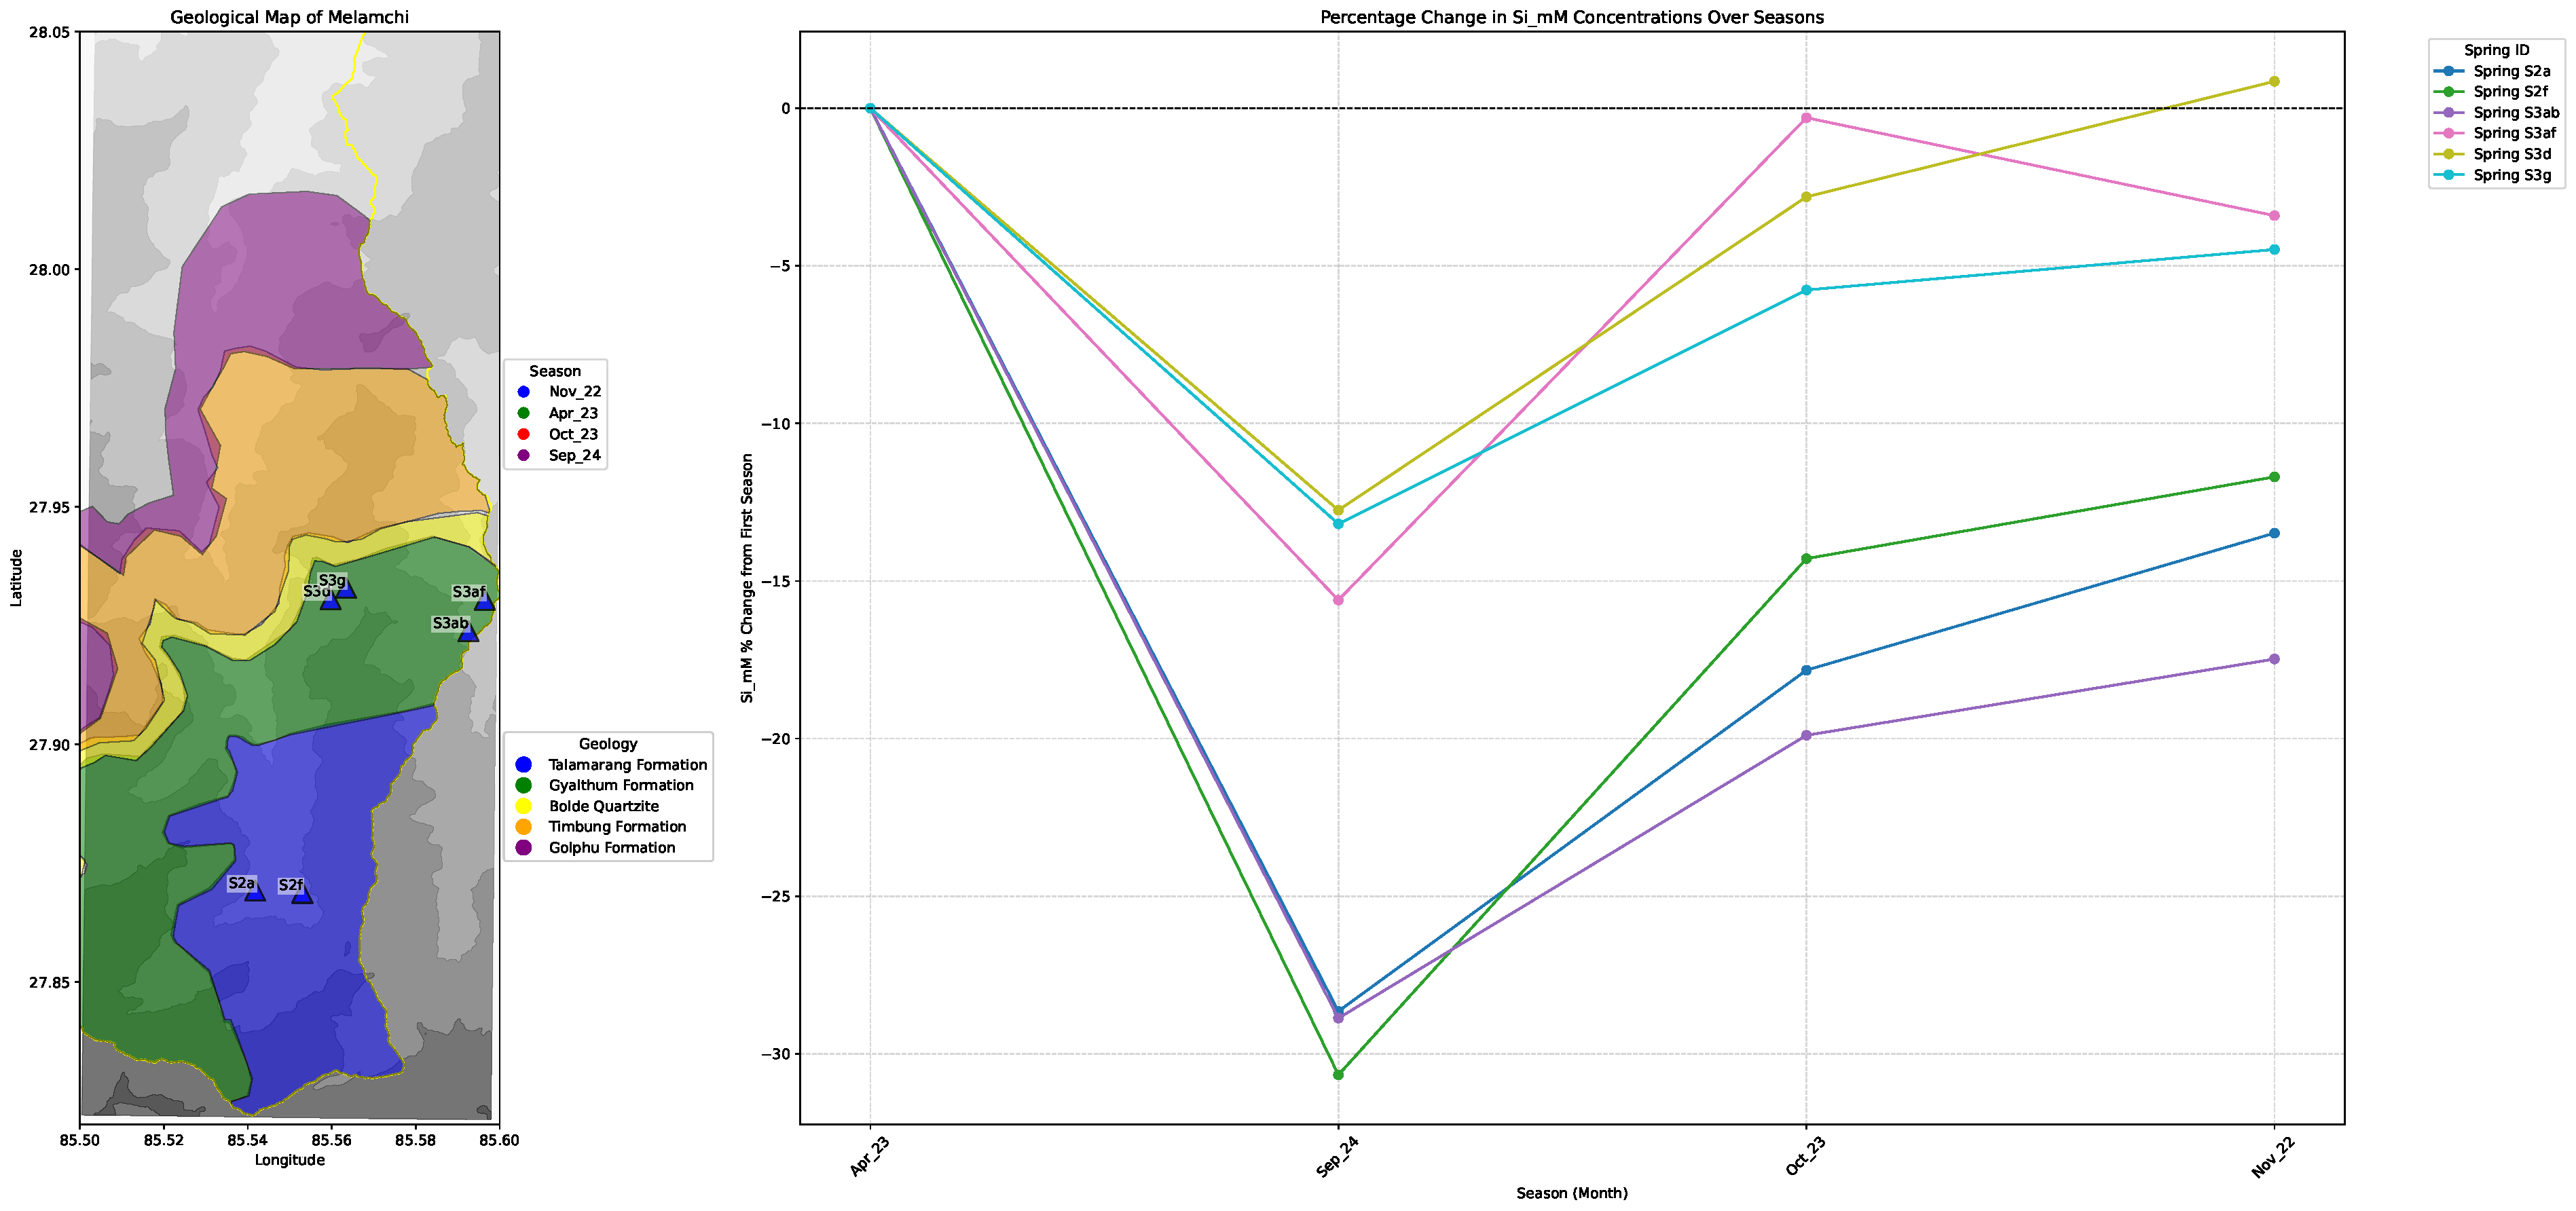
\includegraphics[width=0.8\textwidth]{Si_mM_percentage_change_springs.pdf}
    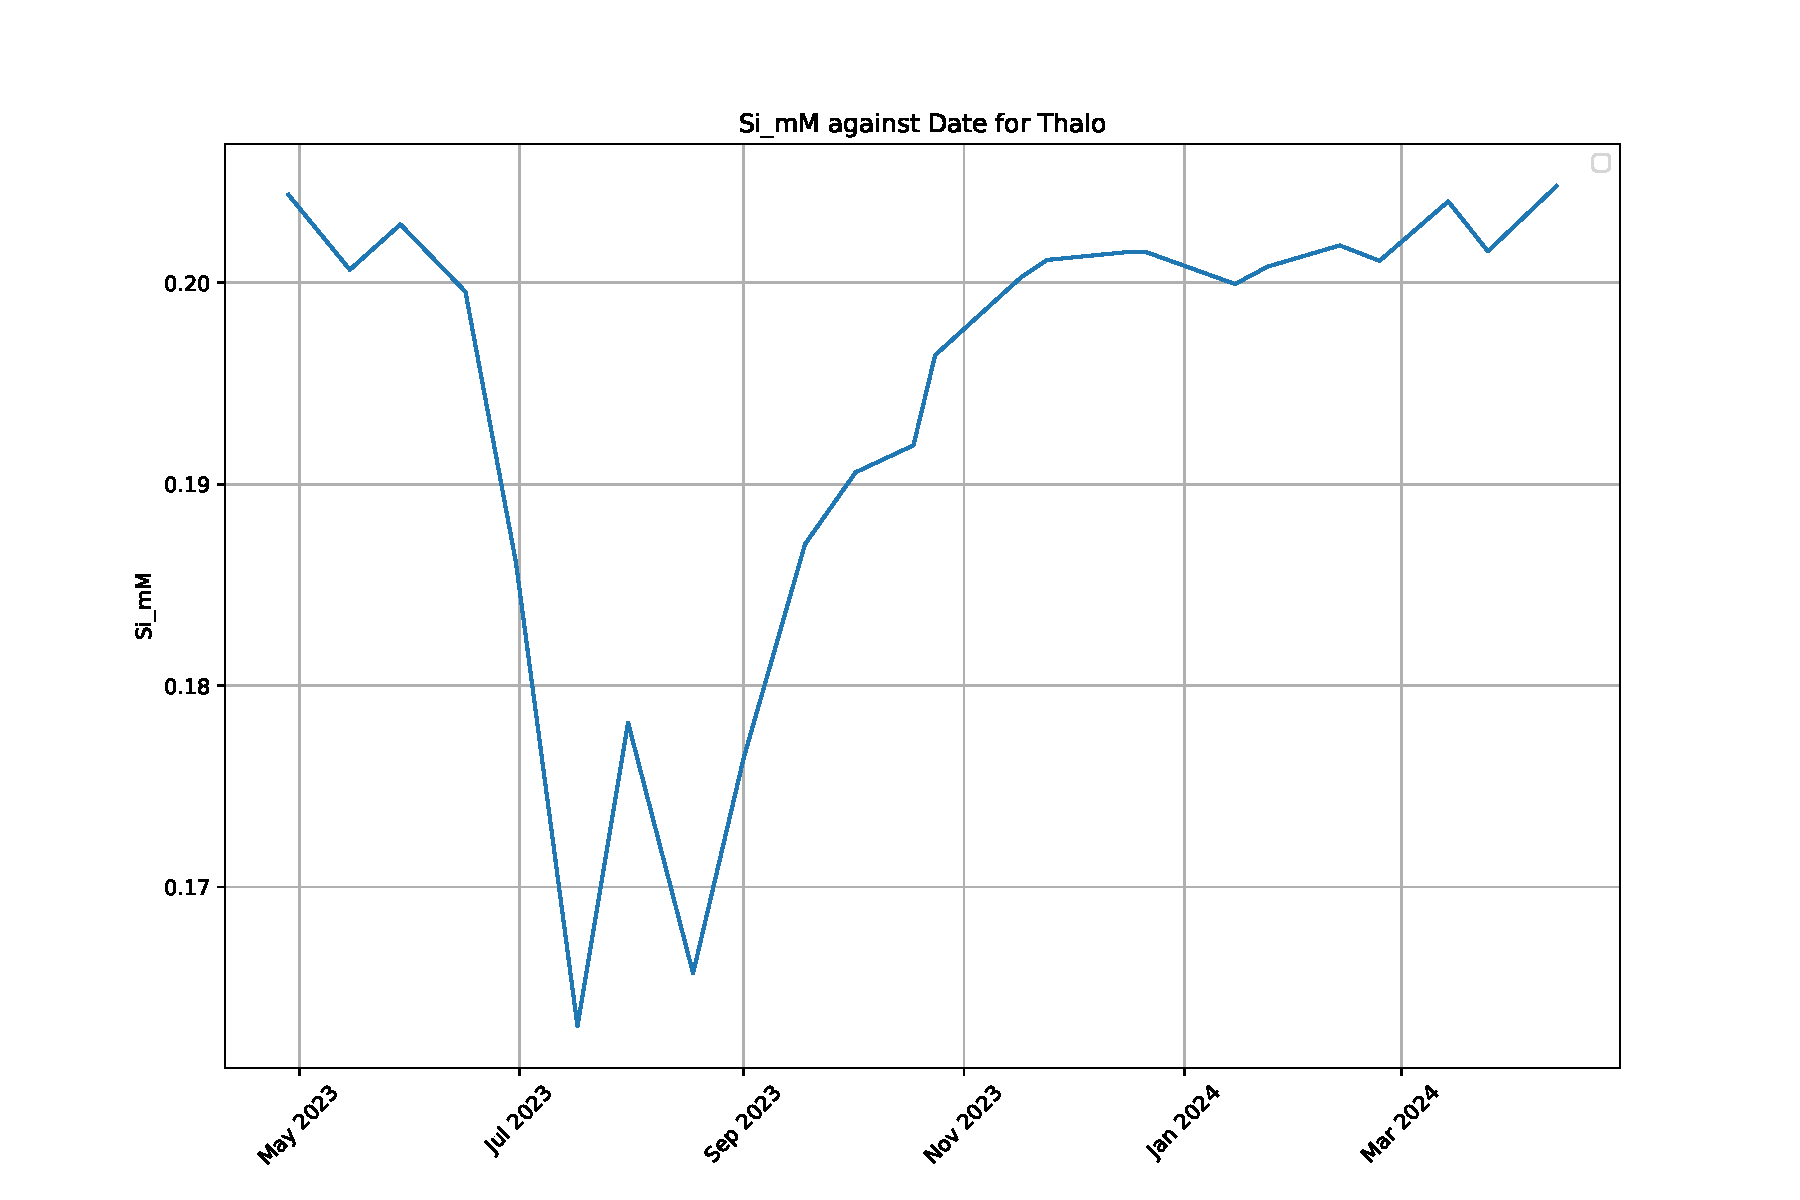
\includegraphics[width=0.8\textwidth]{Si_mM_Thalo_timeseries.pdf}
    \caption{Seasonal changes in spring concentration indicating monsoonal precipitation influence.; Time series of spring concentration changes over time.}
    \label{fig:time_series_changes}
\end{figure}

\FloatBarrier


\subsection{Stronrium Isotope Values of Springs and Rain}



\begin{landscape} % Start landscape mode

    \scriptsize  % Reduce font size for better fit

    \noindent % Avoid indentation
    \begin{minipage}{0.48\linewidth} % First half of the landscape page

        \begin{longtable}{l r r l r r}
            \caption{Strontium isotope values (Part 1)} \label{tab:sr87_sr86_data1} \\
            \hline
            \textbf{Sample ID} & \textbf{Elevation (m)} & \textbf{pH} & \boldmath{$^{87}$Sr/$^{86}$Sr} (\textbf{2SD} $\cdot$10$^{\text{6}}$)} & \textbf{Sr ($\mu$M)} & \textbf{Cl ($\mu$M)} \\
            \hline
            \endfirsthead

            \multicolumn{6}{c}{\textbf{(Continued from previous page)}} \\
            \hline
            \textbf{Sample ID} & \textbf{Elevation (m)} & \textbf{pH} & \boldmath{$^{87}$Sr/$^{86}$Sr} (\textbf{2SD} $\cdot$10$^{\text{6}}$)} & \textbf{Sr ($\mu$M)} & \textbf{Cl ($\mu$M)} \\
            \hline
            \endhead

            \hline
            \multicolumn{6}{r}{\textit{Continued on next column}} \\
            \endfoot

            \hline
            \endlastfoot


            \multicolumn{6}{c}{\textbf{Rain}} \\

            NEP24-039 & 840 & 6.79 & 0.73906 \hfill (24) & 0.13 & 28.09 \\
            NEP24-043 & 1351 & 5.82 & 0.71442 \hfill (46) & 0.01 & 3.55 \\
            NEP24-044 & 1952 & 6.05 & 0.71352 \hfill (127) & 0.01 & 1.89 \\
            NEP24-045 & 2644 & 5.00 & 0.71292 \hfill (73) & 0.01 & 3.21 \\
            NEP24-046 & 2110 & 6.02 & 0.70904 \hfill (100) & 0.02 & 2.86 \\
            NEP24-047 & 2644 & 5.74 & 0.71194 \hfill (237) & 0.01 & 0.55 \\
            NEP24-048 & 2644 & 5.61 & 0.71182 \hfill (189) & 0.01 & 3.65 \\
            \hline

            \multicolumn{6}{c}{\textbf{Traverse 1}} \\
            NEP22-1 & 871 & 7.08 & 0.74101 \hfill (29) & 0.34 & 81.09 \\
            NEP22-2 & 890 & 7.75 & 0.74115 \hfill (22) & 0.35 & 92.95 \\
            NEP22-80 & 1045 & 7.71 & 0.75192 \hfill (33) & 0.26 & 6.43 \\
            NEP22-81 & 1209 & 7.89 & 0.75506 \hfill (27) & 0.21 & 10.64 \\
            NEP22-82 & 1213 & 7.04 & 0.75517 \hfill (23) & 0.31 & 13.10 \\
            NEP22-83 & 1245 & 6.24 & 0.75154 \hfill (27) & 0.31 & 4.31 \\
            NEP22-84 & 1173 & 7.86 & 0.74969 \hfill (61) & 0.28 & 3.17 \\
            NEP22-85 & 1197 & 7.56 & 0.75394 \hfill (32) & 0.16 & 2.38 \\
            NEP22-86 & 1125 & 8.27 & 0.75957 \hfill (35) & 0.07 & 54.46 \\
            NEP22-87 & 1268 & 6.26 & 0.74341 \hfill (25) & 0.78 & 223.01 \\
            \hline
            
            \multicolumn{6}{c}{\textbf{Traverse 2}} \\

            NEP22-61 & 1528 & 5.32 & 0.74691 \hfill (62) & 0.29 & 349.74 \\
            NEP22-62 & 1503 & 6.41 & 0.73943 \hfill (25) & 0.06 & 362.10 \\
            NEP22-63 & 1447 & 6.73 & 0.74943 \hfill (37) & 0.47 & 152.05 \\
            NEP22-64 & 1444 & 6.53 & 0.74872 \hfill (25) & 0.33 & 101.99 \\
            NEP22-65 & 1430 & 6.51 & 0.74886 \hfill (30) & 0.17 & 58.79 \\
            NEP22-66 & 1359 & 7.35 & 0.74629 \hfill (30) & 0.03 & 126.02 \\
            NEP22-67 & 1126 & 6.83 & 0.74510 \hfill (41) & 0.48 & 235.79 \\
            NEP22-68 & 1288 & 5.42 & 0.75696 \hfill (23) & 0.29 & 112.71 \\
            NEP22-70 & 950 & 7.54 & 0.73128 \hfill (37) & 1.18 & 60.86 \\
            NEP22-71 & 996 & 7.99 & 0.74253 \hfill (42) & 0.31 & 125.59 \\
            NEP22-73 & 979 & 6.73 & 0.73191 \hfill (19) & 0.86 & 41.91 \\
            NEP22-75 & 1054 & 6.53 & 0.73921 \hfill (71) & 0.46 & 117.33 \\
            NEP22-76 & 1073 & 6.82 & 0.73701 \hfill (21) & 0.43 & 111.78 \\
            NEP22-78 & 1272 & 6.74 & 0.74584 \hfill (36) & 0.17 & 40.32 \\
            NEP22-79 & 1276 & 5.67 & 0.74752 \hfill (56) & 0.29 & 305.63 \\
            \hline

        \end{longtable}

    \end{minipage} % End first column

    \hfill % Add space between tables

    \begin{minipage}{0.48\linewidth} % Second half of the landscape page

        \begin{longtable}{l r r l r r}
            \caption{Strontium isotope values (Part 2)} \label{tab:sr87_sr86_data2} \\
            \hline
            \textbf{Sample ID} & \textbf{Elevation (m)} & \textbf{pH} & \boldmath{$^{87}$Sr/$^{86}$Sr} (\textbf{2SD} $\cdot$10$^{\text{6}}$)} & \textbf{Sr ($\mu$M)} & \textbf{Cl ($\mu$M)} \\
            \hline
            \endfirsthead

            \multicolumn{6}{c}{\textbf{(Continued from previous page)}} \\
            \hline
            \textbf{Sample ID} & \textbf{Elevation (m)} & \textbf{pH} & \boldmath{$^{87}$Sr/$^{86}$Sr} (\textbf{2SD} $\cdot$10$^{\text{6}}$)} & \textbf{Sr ($\mu$M)} & \textbf{Cl ($\mu$M)} \\
            \hline
            \endhead

            \hline
            \multicolumn{6}{r}{\textit{Continued on next page}} \\
            \endfoot

            \hline
            \endlastfoot

            \multicolumn{6}{c}{\textbf{Traverse 3}} \\

            NEP22-10 & 2419 & 6.48 & 0.73918 \hfill (60) & 0.20 & 17.13 \\
            NEP22-11 & 2419 & 6.59 & 0.73819 \hfill (20) & 0.22 & 15.76 \\
            NEP22-12 & 2390 & 6.77 & 0.73162 \hfill (27) & 0.16 & 2.89 \\
            NEP22-13 & 2099 & 6.76 & 0.73614 \hfill (54) & 0.25 & 9.03 \\
            NEP22-15 & 1975 & 7.29 & 0.73841 \hfill (14) & 0.23 & 4.98 \\
            NEP22-16 & 1967 & 7.14 & 0.73370 \hfill (22) & 0.15 & 1.05 \\
            NEP22-17 & 2100 & 6.90 & 0.73584 \hfill (26) & 0.21 & 11.74 \\
            NEP22-18 & 2091 & 6.98 & 0.73281 \hfill (19) & 0.38 & 8.66 \\
            NEP22-19 & 2095 & 6.07 & 0.73594 \hfill (28) & 0.25 & 9.44 \\
            NEP22-20 & 2104 & 7.14 & 0.73241 \hfill (34) & 0.11 & 6.87 \\
            NEP22-42 & 1325 & 6.24 & 0.73680 \hfill (62) & 0.31 & 27.25 \\
            NEP22-45 & 1194 & 7.57 & 0.73763 \hfill (22) & 0.32 & 23.90 \\
            NEP22-53 & 1776 & 6.33 & 0.73720 \hfill (39) & 0.40 & 19.70 \\
            NEP22-54 & 1781 & 6.19 & 0.73831 \hfill (18) & 0.36 & 20.39 \\
            NEP22-55 & 1771 & 6.69 & 0.73824 \hfill (19) & 0.36 & 19.57 \\
            NEP22-56 & 1433 & 6.86 & 0.74129 \hfill (26) & 0.42 & 23.24 \\
            NEP22-57 & 1464 & 6.85 & 0.73240 \hfill (37) & 0.69 & 46.41 \\
            NEP22-58 & 1447 & 7.34 & 0.73871 \hfill (19) & 0.36 & 7.57 \\
            NEP22-59 & 1324 & 7.48 & 0.73780 \hfill (73) & 0.32 & 14.91 \\
            NEP22-60 & 1161 & 7.04 & 0.73121 \hfill (24) & 0.38 & 22.66 \\
            NEP24-010 & 1314 & 6.45 & 0.73689 \hfill (94) & 0.31 & 21.65 \\
            NEP24-011 & 1319 & 7.07 & 0.73782 \hfill (29) & 0.33 & 10.92 \\
            NEP24-014 & 2496 & 6.58 & 0.73508 \hfill (0) & 0.03 & 1.84 \\
            NEP24-015 & 2104 & 6.10 & 0.73644 \hfill (47) & 0.20 & 7.38 \\
            NEP24-016 & 1978 & 7.05 & 0.73360 \hfill (20) & 0.16 & 0.39 \\
            \hline
            \multicolumn{6}{c}{\textbf{Traverse 4}} \\

            NEP22-46 & 2555 & 7.05 & 0.74922 \hfill (56) & 0.16 & 3.37 \\
            NEP22-47 & 2451 & 6.65 & 0.73661 \hfill (36) & 0.19 & 7.65 \\
            NEP22-48 & 2067 & 6.63 & 0.74727 \hfill (28) & 0.22 & 2.64 \\
            NEP22-49 & 1968 & 6.88 & 0.73730 \hfill (28) & 0.44 & 5.12 \\
            NEP22-50 & 1698 & 6.69 & 0.73508 \hfill (39) & 0.62 & 21.22 \\
            NEP22-52 & 1532 & 7.00 & 0.73828 \hfill (22) & 0.18 & 7.99 \\
            \hline
            \multicolumn{6}{c}{\textbf{Traverse 5}} \\

            NEP22-22 & 2755 & 6.90 & 0.73006 \hfill (20) & 0.19 & 1.94 \\
            NEP22-23 & 2516 & 6.17 & 0.73210 \hfill (26) & 0.13 & 1.19 \\
            NEP22-24 & 2626 & 7.16 & 0.72989 \hfill (20) & 0.19 & 5.93 \\
            NEP22-25 & 2566 & 7.24 & 0.72999 \hfill (44) & 0.24 & 4.23 \\
            NEP22-26 & 2577 & 6.83 & 0.73230 \hfill (22) & 0.11 & 1.73 \\
            NEP22-27 & 3122 & 7.00 & 0.73165 \hfill (35) & 0.09 & 1.53 \\
            NEP22-28 & 2953 & 7.22 & 0.73238 \hfill (26) & 0.11 & 1.73 \\
            NEP22-29 & 2850 & 7.24 & 0.73218 \hfill (22) & 0.15 & 1.71 \\
            NEP22-30 & 2760 & 6.70 & 0.73243 \hfill (24) & 0.17 & 3.08 \\
            NEP22-31 & 2564 & 6.90 & 0.73244 \hfill (25) & 0.28 & 1.96 \\
            NEP22-32 & 2252 & 6.27 & 0.73227 \hfill (23) & 0.26 & 11.19 \\
            NEP22-33 & 2249 & 7.51 & 0.73166 \hfill (20) & 0.26 & 13.14 \\
            NEP22-34 & 2240 & 7.35 & 0.73155 \hfill (56) & 0.27 & 16.81 \\
            NEP22-35 & 2066 & 7.55 & 0.73334 \hfill (19) & 0.16 & 2.78 \\
            NEP22-36 & 1986 & 7.84 & 0.73205 \hfill (20) & 0.27 & 3.00 \\
            NEP22-37 & 2050 & 7.72 & 0.73280 \hfill (44) & 0.22 & 2.33 \\
            NEP22-39 & 2524 & 7.60 & 0.73116 \hfill (22) & 0.18 & 4.51 \\

            \hline
        \end{longtable}

    \end{minipage} % End first column

\end{landscape}


\FloatBarrier


Radiogenic strontium isotope analyses of springs show a wide variation between different traverses. Sr isotopes were also measured for the collected rain samples, and these range from 0.70904 to 0.73906. The lowest of these rain values is close to the reported value for seawater, which is 0.70917.  

\newpage





\section{Discussion}

\subsection{Explaining Traversal Variations in Chemistry}
\label{subsection:trav}

Increasing DSi concentration with decreasing elevation suggests the springs are sampling increasingly longer flow paths. This is because longer flow paths allow for more water-rock interaction, which scavenges more DSi from the silicate rocks. While most traverses show such a trend, this does not happen in Traverse 1. One possible reason is that the lowermost springs are likely to be close to the Melamchi river; this is more dilute than the most concentrated springs in the traverse. Mixing with the river waters is possible but unlikely because of the difference in elevation. It is unlikely that the decrease is caused by a dilution effect at the start of the monsoon such as that shown in Figure \ref{fig:time_series_changes}. This is because these DSi trends are consistent across multiple seasons within error. Clearly, however, samples collected in September will be relatively more dilute than those collected in April.

\bsk

A decrease in DSi at lower elevations here could also suggest precipitation of secondary minerals, which is apparent from the Na$^+$/DSi ratio. Linear trends in plot (b) for Traverses 1, 3, and 5 show an increase in Na$^+$/DSi as elevation decreases. Elevated Na$^+$/DSi is interpreted as a sign of a closer approach to equilibrium. Si is involved in kaolinite precipitation whilst Na$^+$ is not, as evidenced in equation \ref{eq:9}, so an increase in their ratio suggests more kaolinite is precipitating \parencite{gaillardetGlobalSilicateWeathering1999}. Kaolinite precipitation is considered to be the backwards reaction, so its increase points to an approach towards equilibrium.

\bsk

Plots of Na$^+$/DSi against elevation can also be used to infer how consistently a given flow path is sampled. Because Na$^+$/DSi is primarily controlled by the balance of dissolution and reprecipitation, and by extension the average age of water in the flow path, consistency of this value over time points to the same flow path length being sampled for a given rate of reaction. Under the steady state assumption assumption $\partial C/\partial t = 0$ used in the residence time models, the Na/DSi ratio should be constant over time at a given elevation if the same flow path is sampled \parencite{lichtner}. For both Traverse 3 and 5, the Na$^+$/DSi ratio against elevation does not change between different seasons. However, there is a better correlation in Traverse 3 which suggests that the flow paths are more consistently sampled there.



\subsection{Residence Time Agreement with Gas Ages}

As shown in Figures 5-9 (c), predicted residence times in the catchment are consistent between the Maher and Fontorbe Models. Residence times increase as elevation decreases, agreeing with the notion that springs sampled at these lower elevations reflect longer flowpaths. Residence times also generally increase with decreasing traversal number, such that Traverse 5 has the lowest and Traverse 1 has the highest. Consistently increasing residence times like this could suggest catchment-wide plumbing, whereby traversal flow paths are interconnected.

\bsk

Residence times in Traverse 3 can be directly compared to the gas ages obtained by \textcite{atwoodCriticalZoneResponse2023}, because both studies are sampling the same springs. The \textcite{atwoodCriticalZoneResponse2023} ages in Traverse 3 range from 5-35 years. The findings from this study and both models predict residence times of a similar order of magnitude. This study does predict older times at the lowest elevation, but these are mostly within the range of propagated uncertainty. Using spring chemistry is therefore a viable method to determine residence times in natural catchments, with the premise that the model assumptions are valid. In addition, this study lends credibility to the use of gas ages to determine residence times, which is an approach that is often criticised for using biased age distributions \parencite{mccallumLimitationsUseEnvironmental2015}. Findings of residence times on the order of 10-100 years for the whole catchment also inform precipitation-discharge relationships. If this study's findings are correct, then the delay in river discharge found by \textcite{andermannImpactTransientGroundwater2012} is likely only recording surface or near-surface flow. The shorter flow paths here could plausibly be associated to residence times of a few months.

\bsk

The fact that both the kinetic-dependent rate Maher model and the kinetics-independent rate Fontorbe model agree with \textcite{atwoodCriticalZoneResponse2023} suggests that the groundwater in Traverse 3 does not get near equilibrium. Reaction rate is kept constant in the Fontorbe model assuming a far from equilibrium state. In the Maher model, reaction rate depends on the equilibrium concentration. As this concentration is reached in the Maher model, the reaction rate will decrease. When the system is far from equilibrium, both models will predict similar times. In order to do test this further, the free energy of the system can be calculated.


\subsection{Free Energy Calculations Concur on Far From Equilibrium State}

\textcite{maherRoleFluidResidence2011} uses their model to conclude that all flow paths reach equilibrium. The free energy of reaction, calculated using the activity of the ions in solution, can be used in natural systems to determine the extent to which equilibrium is reached (\cite{kampmanFeldsparDissolutionKinetics2009}; \cite{wojtowiczThermodynamicBasisSaturation}). Free energies lower than -10 kJ/mol are considered close to equilibrium, whilst those more negative than -40 kJ/mol are categorised as far from equilibrium \parencite{kampmanFeldsparDissolutionKinetics2009}. This method can therefore test the validity of the Maher model in Melamchi. Free energy is defined as:

\begin{equation}
    \Delta G = \Delta G^0 + RT \ln Q
    \label{eq:deltag}
\end{equation}\\

Where in equation \ref{eq:deltag}, $\Delta G$ represents the Gibbs free energy change of reaction, $\Delta G^0$ is the standard Gibbs free energy change, $R$ is the universal gas constant, $T$ denotes the absolute temperature in kelvins, and $Q$ is the reaction quotient. As discussed in the Methods \ref{subsection:weathering}, the weathering reaction characterising this catchment is the dissolution of plagioclase (An-20) and the precipitation of kaolinite, given by equation \ref{eq:9}. The exact composition of plagioclase is important for these calculations. The free energy of reaction is lowered by the presence of a solid solution between albite and anorthite \parencite{dubacqThermodynamicsOrderingMixing2022}. The parameters for the standard free energy of reaction are calculated using the pygcc python package \parencite{awolayoPyGeochemCalcPython2022}. The package gives the standard properties of solid-solution species and reactions, such that $\Delta G^0$ can be calculated:

\begin{equation}
    \Delta G^0 = \Delta G^0_{products} - \Delta G^0_{reactants} = -RT \ln K
\end{equation}

K is calculated using the database obtained from pygcc using The Geochemist's Workbench® Rxn program \parencite{bethkeGEOCHEMICALBIOGEOCHEMICALREACTION}. Q is calculated as the ion activity product of the reaction, assuming the activities of the solid phases plagioclase and kaolinite are 1, the activity of water is 1, and the activity of the ions in solution are equal to their concentration.

\begin{equation}
    Q = \frac{a_{\mathrm{Kaol}}^{0.6}\,a_{\mathrm{Na}^{+}}^{0.8}\,a_{\mathrm{Ca}^{2+}}^{0.2}\,a_{\mathrm{SiO_{2}(aq)}}^{1.6}}
           {a_{\mathrm{An_{20}}}\,a_{\mathrm{H}^{+}}^{1.2}}
\end{equation}


\begin{figure}[H]
    \centering
    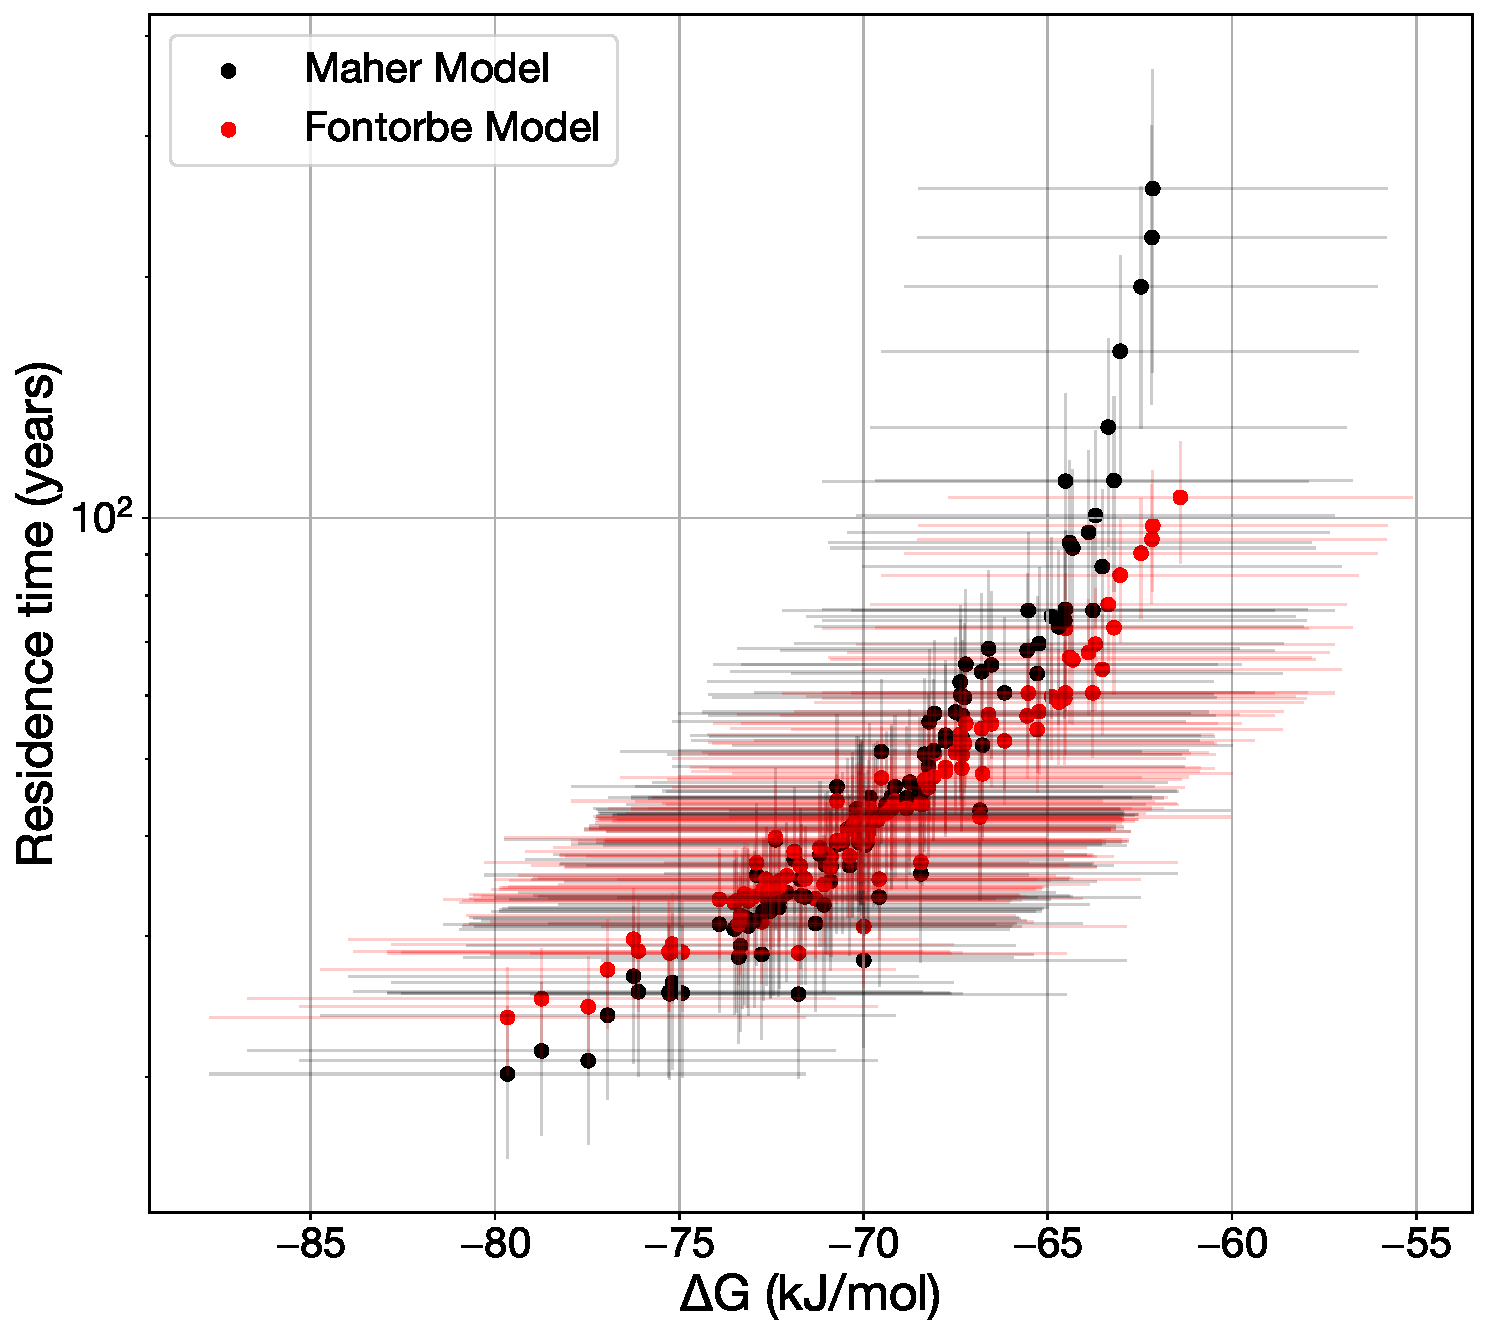
\includegraphics[width=0.8\textwidth]{DGMF.pdf}
    \caption{Estimated residence time against calculated free energy of reaction. Error bars represent Monte Carlo propagated uncertainty. Red points plot the Fontorbe model, while black points plot the Maher model.}
    \label{fig:deltag}
\end{figure}

\FloatBarrier

Figure \ref{fig:deltag} shows that all springs in the catchment have a free energy that is more negative than -60 kJ/mol. These samples are therefore classified as far from equilibrium. Note that being far from equilibrium is not inconsistent with evidence for secondary precipitation as shown in Figures \ref{fig:modal}, \ref{fig:trav1}-\ref{fig:trav5}; simply, being closer to equilibrium would suggest more precipitation. Figure \ref{fig:deltag} does show that free energy gets closer to zero as residence time increases. This is consistent with the notion that groundwaters approach equilibrium the more they stay in the subsurface and react. However, the extent of reaction is not great enough to be considered close to equilibrium. This suggests that, for Melamchi, using the Maher model to estimate residence times is not appropriate.


% \caption{Summary of free energy results from each traverse. Standard deviation corresponds to Monte Carlo propagated uncertainty.} \\
% \label{tab:delta_G}\\

% Begin two-column layout


\begin{landscape}
    
    \begin{table}
        \caption{Summary of free energy results from each traverse. Standard deviation corresponds to Monte Carlo propagated uncertainty.}
        \label{tab:delta_G}
        \scriptsize  % Apply scriptsize to the entire table
        \setlength\tabcolsep{2mm}
        \begin{tabular}{M{.30\textwidth} @{\hspace{4cm}} M{.30\textwidth} @{\hspace{4cm}} M{.30\textwidth}}
            % First column - Transactions Table
            \begin{tabular}{l l l l l}
    \textbf{Sample ID}  &  \textbf{Season}  &  \textbf{Traverse}  &  \textbf{Elevation}  &  \textbf{$\Delta$G $\pm$ 1$\sigma$} \\
    \hline
    &   &   &  \textbf{m}  &  \textbf{kJ/mol} \\
    \hline
    NEP24-001 & Sep 24 & Traverse 1 & 928 & -69.7 ±  7.1 \\
    NEP22-87 & Nov 22 & Traverse 1 & 1270 & -68.5 ±  7.0 \\
    MKS 1B & Nov 18 & Traverse 1 & 1432 & -68.2 ±  7.0 \\
    NEP22-86 & Nov 22 & Traverse 1 & 1124 & -66.5 ±  6.8 \\
    NEP24-003 & Sep 24 & Traverse 1 & 876 & -65.6 ±  6.7 \\
    NEP22-2 & Nov 22 & Traverse 1 & 890 & -65.3 ±  6.7 \\
    MKS-1 & Nov 18 & Traverse 1 & 1433 & -64.6 ±  6.6 \\
    NEP24-002 & Sep 24 & Traverse 1 & 868 & -64.6 ±  6.6 \\
    NEP22-85 & Nov 22 & Traverse 1 & 1195 & -64.5 ±  6.6 \\
    MKS-3 & Nov 18 & Traverse 1 & 1152 & -64.4 ±  6.6 \\
    NEP22-1 & Nov 22 & Traverse 1 & 871 & -63.8 ±  6.5 \\
    MKS-24 & Nov 18 & Traverse 1 & 850 & -63.6 ±  6.5 \\
    NEP22-80 & Nov 22 & Traverse 1 & 1046 & -63.4 ±  6.5 \\
    NEP22-81 & Nov 22 & Traverse 1 & 1207 & -63.1 ±  6.4 \\
    NEP22-82 & Nov 22 & Traverse 1 & 1212 & -62.5 ±  6.4 \\
    NEP22-83 & Nov 22 & Traverse 1 & 1244 & -62.3 ±  6.4 \\
    MKS-2 & Nov 18 & Traverse 1 & 1083 & -62.2 ±  6.4 \\
    \specialrule{0.2pt}{1pt}{1pt}
    NEP24-061 & Sep 24 & Traverse 2 & 1527 & -76.4 ±  7.8 \\
    NEP22-61 & Nov 22 & Traverse 2 & 1524 & -76.3 ±  7.7 \\
    NEP24-062 & Sep 24 & Traverse 2 & 1452 & -72.5 ±  7.4 \\
    NEP22-62 & Nov 22 & Traverse 2 & 1504 & -71.8 ±  7.3 \\
    NEP22-79 & Nov 22 & Traverse 2 & 1277 & -71.8 ±  7.3 \\
    NEP22-63 & Nov 22 & Traverse 2 & 1447 & -71.4 ±  7.3 \\
    NEP22-66 & Nov 22 & Traverse 2 & 1359 & -71.0 ±  7.2 \\
    \hline
    \end{tabular}
    &
    % Second column
    \begin{tabular}{l l l l l}
        \setlength\tabcolsep{0.1cm}
\textbf{Sample ID}  &  \textbf{Season}  &  \textbf{Traverse}  &  \textbf{Elevation}  &  \textbf{$\Delta$G $\pm$ 1$\sigma$} \\
\hline
&   &   &  \textbf{m}  &  \textbf{kJ/mol} \\
\hline
    NEP22-65 & Nov 22 & Traverse 2 & 1429 & -70.8 ±  7.2 \\
    NEP24-065 & Sep 24 & Traverse 2 & 1129 & -70.1 ±  7.1 \\
    NEP24-063 & Sep 24 & Traverse 2 & 1285 & -68.8 ±  7.0 \\
    NEP22-64 & Nov 22 & Traverse 2 & 1442 & -68.3 ±  7.0 \\
    NEP22-78 & Nov 22 & Traverse 2 & 1270 & -67.5 ±  6.9 \\
    NEP22-68 & Nov 22 & Traverse 2 & 1288 & -67.4 ±  6.9 \\
    NEP22-67 & Nov 22 & Traverse 2 & 1125 & -66.9 ±  6.8 \\
    NEP24-068 & Sep 24 & Traverse 2 & 949 & -66.9 ±  6.8 \\
    NEP22-77 & Nov 22 & Traverse 2 & 1273 & -66.7 ±  6.8 \\
    NEP24-067 & Sep 24 & Traverse 2 & 1000 & -66.2 ±  6.8 \\
    NEP22-71 & Nov 22 & Traverse 2 & 996 & -65.3 ±  6.7 \\
    MKS-10 & Nov 18 & Traverse 2 & 930 & -65.0 ±  6.7 \\
    NEP22-70 & Nov 22 & Traverse 2 & 950 & -64.8 ±  6.6 \\
    MKS 10B & Nov 18 & Traverse 2 & 929 & -64.6 ±  6.6 \\
    NEP22-76 & Nov 22 & Traverse 2 & 1074 & -64.0 ±  6.6 \\
    NEP22-75 & Nov 22 & Traverse 2 & 1052 & -63.8 ±  6.5 \\
    NEP22-73 & Nov 22 & Traverse 2 & 979 & -63.2 ±  6.5 \\
    \specialrule{0.2pt}{1pt}{1pt}
    NEP24-014 & Sep 24 & Traverse 3 & 2496 & -79.8 ±  8.1 \\
    NEP22-9 & Nov 22 & Traverse 3 & 2522 & -78.9 ±  8.0 \\
    NEP24-015 & Sep 24 & Traverse 3 & 2101 & -75.1 ±  7.6 \\
    NEP24-016 & Sep 24 & Traverse 3 & 1979 & -75.0 ±  7.7 \\
    NEP24-034 & Sep 24 & Traverse 3 & 2415 & -74.9 ±  7.6 \\
    MKS-6 & Nov 18 & Traverse 3 & 2124 & -74.6 ±  7.6 \\
    NEP22-20 & Nov 22 & Traverse 3 & 2104 & -74.6 ±  7.6 \\
    \hline
        \end{tabular}
        &
        % Second column
        \begin{tabular}{l l l l l}
            \setlength\tabcolsep{0.1cm}
    \textbf{Sample ID}  &  \textbf{Season}  &  \textbf{Traverse}  &  \textbf{Elevation}  &  \textbf{$\Delta$G $\pm$ 1$\sigma$} \\
    \hline
    &   &   &  \textbf{m}  &  \textbf{kJ/mol} \\
    \hline
    NEP22-17 & Nov 22 & Traverse 3 & 2102 & -74.0 ±  7.5 \\
    NEP22-12 & Nov 22 & Traverse 3 & 2386 & -73.6 ±  7.5 \\
    NEP22-16 & Nov 22 & Traverse 3 & 1964 & -73.4 ±  7.5 \\
    NEP22-19 & Nov 22 & Traverse 3 & 2097 & -73.4 ±  7.5 \\
    NEP22-13 & Nov 22 & Traverse 3 & 2098 & -73.2 ±  7.5 \\
    NEP22-10 & Nov 22 & Traverse 3 & 2418 & -73.1 ±  7.4 \\
    NEP22-11 & Nov 22 & Traverse 3 & 2418 & -73.0 ±  7.4 \\
    NEP22-46 & Nov 22 & Traverse 3 & 2555 & -72.8 ±  7.4 \\
    MKS 5B & Nov 18 & Traverse 3 & 2428 & -72.5 ±  7.4 \\
    MKS-5 & Nov 18 & Traverse 3 & 2434 & -72.0 ±  7.3 \\
    NEP24-017 & Sep 24 & Traverse 3 & 1990 & -71.8 ±  7.3 \\
    NEP22-15 & Nov 22 & Traverse 3 & 1973 & -70.2 ±  7.2 \\
    NEP22-18 & Nov 22 & Traverse 3 & 2091 & -70.2 ±  7.2 \\
    NEP24-011 & Sep 24 & Traverse 3 & 1318 & -70.1 ±  7.1 \\
    NEP24-010 & Sep 24 & Traverse 3 & 1314 & -70.0 ±  7.1 \\
    MKS-7 & Nov 18 & Traverse 3 & 1805 & -69.8 ±  7.1 \\
    NEP22-55 & Nov 22 & Traverse 3 & 1772 & -69.8 ±  7.1 \\
    NEP22-54 & Nov 22 & Traverse 3 & 1779 & -69.7 ±  7.1 \\
    NEP22-59 & Nov 22 & Traverse 3 & 1324 & -69.5 ±  7.1 \\
    NEP22-53 & Nov 22 & Traverse 3 & 1777 & -69.4 ±  7.0 \\
    NEP22-42 & Nov 22 & Traverse 3 & 1325 & -69.3 ±  7.1 \\
    NEP22-60 & Nov 22 & Traverse 3 & 1160 & -68.5 ±  7.0 \\
    MKS-9 & Nov 18 & Traverse 3 & 1212 & -68.4 ±  7.0 \\
    MKS 9B & Nov 18 & Traverse 3 & 1214 & -67.8 ±  6.9 \\
    \hline
        \end{tabular}\\ % Correct placement of hline after the main row
    \end{tabular}
\end{table}
\end{landscape}

   \newpage

   \begin{landscape}
    
    \begin{table}
        \scriptsize  % Apply scriptsize to the entire table
        \setlength\tabcolsep{2mm}
        \begin{tabular}{M{.30\textwidth} @{\hspace{4cm}} M{.30\textwidth} @{\hspace{4cm}} M{.30\textwidth}}
            % First column - Transactions Table
            \begin{tabular}{l l l l l}
            \textbf{Sample ID}  &  \textbf{Season}  &  \textbf{Traverse}  &  \textbf{Elevation}  &  \textbf{$\Delta$G $\pm$ 1$\sigma$} \\
            \hline
            &   &   &  \textbf{m}  &  \textbf{kJ/mol} \\
            \hline
    NEP22-45 & Nov 22 & Traverse 3 & 1195 & -67.8 ±  6.9 \\
    NEP24-038 & Sep 24 & Traverse 3 & 1408 & -67.6 ±  6.9 \\
    MKS-8 & Nov 18 & Traverse 3 & 1430 & -67.4 ±  6.9 \\
    NEP22-58 & Nov 22 & Traverse 3 & 1447 & -67.4 ±  6.9 \\
    NEP22-56 & Nov 22 & Traverse 3 & 1433 & -66.9 ±  6.8 \\
    \specialrule{0.2pt}{1pt}{1pt}
    MKS 4B & Nov 18 & Traverse 4 & 2524 & -76.3 ±  7.8 \\
    NEP24-050 & Sep 24 & Traverse 4 & 2452 & -73.6 ±  7.5 \\
    NEP22-48 & Nov 22 & Traverse 4 & 2067 & -71.1 ±  7.2 \\
    NEP24-051 & Sep 24 & Traverse 4 & 2076 & -71.0 ±  7.3 \\
    NEP24-041 & Sep 24 & Traverse 4 & 1614 & -70.8 ±  7.2 \\
    MKS-13 & Nov 18 & Traverse 4 & 2077 & -70.7 ±  7.2 \\
    NEP22-47 & Nov 22 & Traverse 4 & 2450 & -70.5 ±  7.2 \\
    MKS-4 & Nov 18 & Traverse 4 & 2521 & -70.3 ±  7.2 \\
    NEP22-52 & Nov 22 & Traverse 4 & 1529 & -69.6 ±  7.1 \\
    NEP24-052 & Sep 24 & Traverse 4 & 1987 & -69.2 ±  7.1 \\
    MKS-12 & Nov 18 & Traverse 4 & 1479 & -68.5 ±  7.0 \\
    NEP22-49 & Nov 22 & Traverse 4 & 1966 & -68.5 ±  7.0 \\
    NEP22-50 & Nov 22 & Traverse 4 & 1698 & -67.4 ±  6.9 \\
    NEP24-040 & Sep 24 & Traverse 4 & 1693 & -67.3 ±  6.9 \\
    NEP22-57 & Nov 22 & Traverse 4 & 1462 & -65.6 ±  6.7 \\
    \specialrule{0.2pt}{1pt}{1pt}
    NEP24-027 & Sep 24 & Traverse 5 & 2858 & -77.6 ±  7.9 \\
    MKS-23 & Nov 18 & Traverse 5 & 3379 & -77.0 ±  7.8 \\
    MKS 21B & Nov 18 & Traverse 5 & 3007 & -76.2 ±  7.7 \\
    NEP22-26 & Nov 22 & Traverse 5 & 2579 & -75.4 ±  7.7 \\
    \hline
    \end{tabular}
    &
    % Second column
    \begin{tabular}{l l l l l}
        \setlength\tabcolsep{0.1cm}

            \textbf{Sample ID}  &  \textbf{Season}  &  \textbf{Traverse}  &  \textbf{Elevation}  &  \textbf{$\Delta$G $\pm$ 1$\sigma$} \\
            \hline
            &   &   &  \textbf{m}  &  \textbf{kJ/mol} \\
            \hline
    NEP22-27 & Nov 22 & Traverse 5 & 3126 & -75.3 ±  7.6 \\
    NEP22-28 & Nov 22 & Traverse 5 & 2954 & -75.3 ±  7.7 \\
    MKS-14 & Nov 18 & Traverse 5 & 2536 & -73.5 ±  7.5 \\
    NEP24-020 & Sep 24 & Traverse 5 & 2556 & -73.5 ±  7.5 \\
    NEP24-028 & Sep 24 & Traverse 5 & 2782 & -73.2 ±  7.4 \\
    NEP22-29 & Nov 22 & Traverse 5 & 2852 & -73.0 ±  7.4 \\
    NEP22-23 & Nov 22 & Traverse 5 & 2517 & -72.9 ±  7.4 \\
    MKS-20 & Nov 18 & Traverse 5 & 1903 & -72.7 ±  7.4 \\
    NEP22-39 & Nov 22 & Traverse 5 & 2523 & -72.6 ±  7.4 \\
    NEP24-025 & Sep 24 & Traverse 5 & 3127 & -72.6 ±  7.4 \\
    NEP22-24 & Nov 22 & Traverse 5 & 2622 & -72.5 ±  7.4 \\
    MKS 22B & Nov 18 & Traverse 5 & 3130 & -72.4 ±  7.4 \\
    NEP22-22 & Nov 22 & Traverse 5 & 2758 & -72.4 ±  7.4 \\
    MKS-22 & Nov 18 & Traverse 5 & 3126 & -72.2 ±  7.4 \\
    NEP22-25 & Nov 22 & Traverse 5 & 2562 & -71.8 ±  7.3 \\
    NEP22-30 & Nov 22 & Traverse 5 & 2757 & -71.7 ±  7.3 \\
    NEP24-022 & Sep 24 & Traverse 5 & 2259 & -71.3 ±  7.3 \\
    NEP22-35 & Nov 22 & Traverse 5 & 2068 & -71.1 ±  7.3 \\
    MKS-17 & Nov 18 & Traverse 5 & 2163 & -71.0 ±  7.2 \\
    MKS 15B & Nov 18 & Traverse 5 & 2000 & -70.4 ±  7.2 \\
    NEP22-32 & Nov 22 & Traverse 5 & 2252 & -70.4 ±  7.2 \\
    NEP24-023 & Sep 24 & Traverse 5 & 2269 & -70.4 ±  7.2 \\
    NEP24-021 & Sep 24 & Traverse 5 & 2243 & -70.3 ±  7.2 \\
    MKS-18 & Nov 18 & Traverse 5 & 2262 & -70.2 ±  7.1 \\
    \hline
    \end{tabular}
    &
    % Second column
    \vtop{
    \begin{tabular}{l l l l l}
        \setlength\tabcolsep{0.1cm}
    \textbf{Sample ID}  &  \textbf{Season}  &  \textbf{Traverse}  &  \textbf{Elevation}  &  \textbf{$\Delta$G $\pm$ 1$\sigma$} \\
    \hline
    &   &   &  \textbf{m}  &  \textbf{kJ/mol} \\
    \hline

    NEP22-33 & Nov 22 & Traverse 5 & 2247 & -70.2 ±  7.1 \\
    MKS 18B & Nov 18 & Traverse 5 & 2265 & -70.1 ±  7.1 \\
    NEP22-31 & Nov 22 & Traverse 5 & 2573 & -70.1 ±  7.1 \\
    NEP22-34 & Nov 22 & Traverse 5 & 2240 & -70.1 ±  7.1 \\
    MKS-16 & Nov 18 & Traverse 5 & 1942 & -70.0 ±  7.1 \\
    MKS-19 & Nov 18 & Traverse 5 & 2164 & -69.9 ±  7.2 \\
    NEP22-37 & Nov 22 & Traverse 5 & 2050 & -69.0 ±  7.0 \\
    NEP22-36 & Nov 22 & Traverse 5 & 1987 & -68.1 ±  6.9 \\
    \hline
        \end{tabular}}\\ % Correct placement of hline after the main row
    \end{tabular}
\end{table}
\end{landscape}

   \newpage


\subsection{Model Sensitivity to Concentration}

Residence times in Traverse 1 are explainably the longest in the catchment. The springs here at are the lowest elevation, so the flow paths are presumably the longest. This is consistent with the highest DSi concentration of the catchment, and evidence for secondary precipitation of kaolinite at the lowest elevations (see Figure \ref{fig:trav1} (b)). In Traverse 1, the Fontorbe model predicts a peak of $\approx$ 100 years, while the Maher model has a much higher residence time of $\approx$ 300 years. The discrepancy is likely due to how the models are formulated.

\begin{table}[h]
    \centering
    \renewcommand{\arraystretch}{2.2} % Adjust row spacing
    \begin{tabular}{cc}
        \toprule
        \textbf{Fontorbe} & \textbf{Maher} \\
        \midrule
        $\displaystyle T_f  = \frac{\left(C_h - C_o\right)\cdot\phi}{\left(1-f\right)\cdot R_n}$ & 
        $\displaystyle T_f = \frac{C_{eq} \cdot \left(C - C_0\right)}{e^2 R_n \left( C_{\text{eq}} - C \right)}$ \\ [10pt]
        \bottomrule
    \end{tabular}
    \caption{Comparison of residence time equations from Fontorbe and Maher.}
    \label{tab:equations}
\end{table}

The difference in the models comes from the underlying assumptions of reaction rate and how it changes towards equilibrium. The Fontorbe assumption that reaction rate remains constant as the reaction progresses is unrealistic, as all weathering reactions are bound to stop at some time. Hence, the Maher model more accurately reflects water in these catchments that is closer to equilibrium. The $\frac{C_{eq}}{(C_{eq} - C)}$ term in the Maher model gets larger as the concentration approaches equilibrium. As a result of this, the Maher model consistently predicts longer residence times than the Fontorbe Model at higher DSi concentrations, while the opposite is true at lower DSi concentrations. For Traverse 1 the $\frac{C_{eq}}{(C_{eq} - C)}$ term grows arbitrarily large, hence the strong discrepancy found in Figure \ref{fig:trav1} (c).

\bsk

For this study's calculations, the equilibrium concentration is taken to be the highest in the catchment, 869 $\mu$M DSi. This concentration corresponds the highest spring concentration found in Traverse 1. Note that in the \textcite{maherHydrologicRegulationChemical2014} model setup, an equilibrium concentration of 375$\mu$M DSi is chosen from the global river data of \textcite{gaillardetGlobalSilicateWeathering1999}. This is sound for a theoretical model but is not appropriate for this catchment. It is unclear, however, whether choosing the highest DSi concentration in the catchment is appropriate. Clearly as this concentration is approached, the Maher model will predict unrealistic residence times, as shown in Figure \ref{fig:deltag}. The free energy of the system suggests the spring system is far away from equilibrium, so choosing a larger $C_{eq}$ would produce better agreement with the Fontorbe model at higher DSi concentrations and allow for the calculated free energy. Additionally, \textcite{maherRoleFluidResidence2011} details several ways in which $C_{eq}$ could change depending on the conditions. For example, increasing pCO$_2$ would increase the concentration of DSi at equilibrium. Another way to potentially estimate the maximum DSi concentration would be to calculate this at equilibrium by simulating further reaction of the most reacted springs with the appropriate minerals. The only assumption here would be that CO$_2$ is conserved. However, if the Maher model assumes that all flow paths reach equilibrium, it is appropriate to use a concentration measured within the catchment; otherwise, applying the model would be of little relevance to the overall discussion on weathering controls.

\begin{figure}[h]
    \centering
    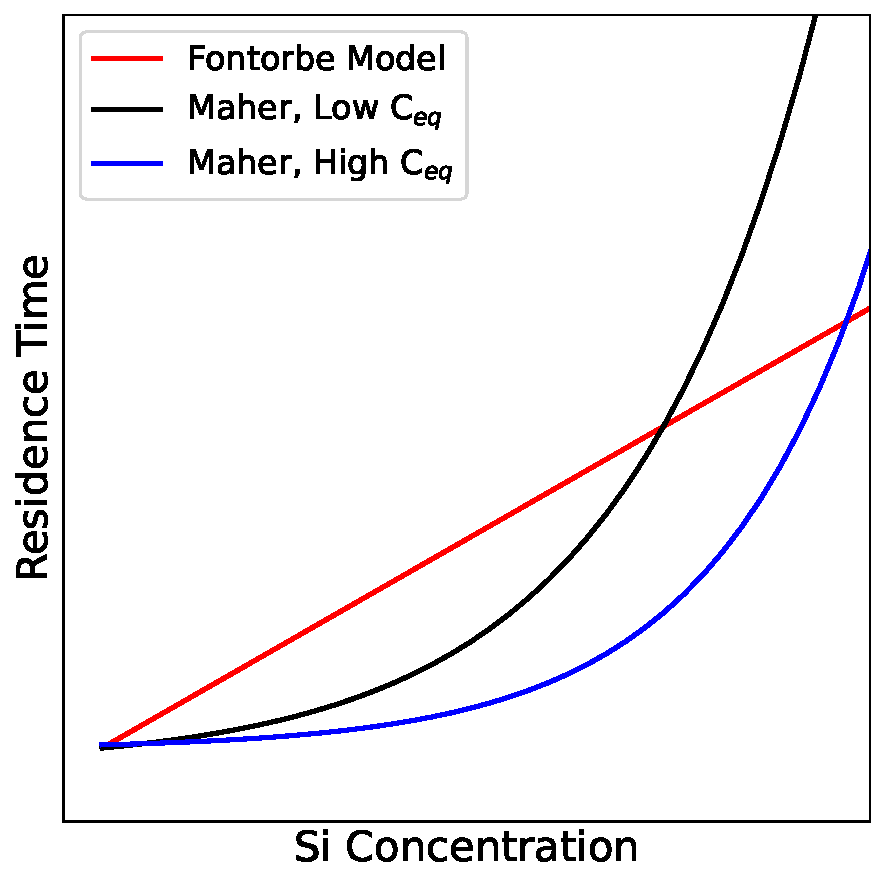
\includegraphics[width=0.6\textwidth]{Linear_vs_Exponential_Comparison.pdf}
    \caption{Illustrative sketch of how dissolved silica concentration changes with flow path length for the two models, and different equilibrium concentration for the Maher model. Plotted lines are taken from the model equations \ref{eq:fontorbe} and \ref{eq:maher}.}
    \label{fig:comparisonceq}
\end{figure}

\FloatBarrier

There is another potential issue related to the dependence of residence time on the concentration of DSi. As is apparent in Figures \ref{fig:trav1}-\ref{fig:trav5} and Table \ref{tab:equations}, the estimated residence time of both models is directly related to the DSi concentration in the spring water. This is by design, however as expressed in subsection \ref{subsection:trav}, low DSi is not necessarily indicative of less reacted groundwater. As a result of this, there is the possibility that the estimated residence times act more as a lower bound. A better approach in a future study could use elemental ratios, for example Na$^+$/DSi that has a known behaviour as the reaction progresses. Elemental ratios like that would also factor out dilution as a potential influencing factor.


\subsection{Is the Rate Constant Used Appropriate?}

Figure \ref{fig:deltag} suggests that the system is far away from equilibrium, but the reaction rate constant used in both models for all calculations is one that is only considered feasible when close to equilibrium \parencite{kampmanFeldsparDissolutionKinetics2009}. In systems far from equilibrium, the reaction rate constant has been suggested to be much larger than those used in the models \parencite{whiteEffectTimeWeathering2003}. Field rate constants lie between 10$^{-13}$ and 10$^{-17}$ mol m$^{-2}$ s$^{-1}$, while laboratory rate constants are between 10$^{-11}$ and 10$^{-13}$ mol m$^{-2}$ s$^{-1}$ \parencite{whiteEffectTimeWeathering2003}. If the rate constant is increased, the residence times predicted by the models will decrease. This is because the rate of reaction is inversely proportional to the residence time, as seen in the equations in Table \ref{tab:equations}. Reaction rate constants that are suggested to be far from equilibrium in \textcite{kampmanFeldsparDissolutionKinetics2009} are laboratory-derived rates, and four orders of magnitude higher than those used in this study. Using these rates for the models predicts residence times in the range of 1-10 days. Under the assumption that the rates displayed in \textcite{kampmanFeldsparDissolutionKinetics2009} are accurate for systems far away from equilibrium, the results no longer agree with \textcite{atwoodCriticalZoneResponse2023}. Under these circumstances, then, the Maher and Fontorbe models are less likely to be appropriate for use in discussing weathering controls. 

\bsk

There are, however, counterarguments to this. Firstly, \textcite{kampmanFeldsparDissolutionKinetics2009} investigate river - not spring - water draining a different lithology, under different pH and pCO$_2$ conditions than Melamchi. Secondly, the reaction rate constants reported at far from equilibrium free energies are calculated in the laboratory, at different conditions to both this study and \textcite{kampmanFeldsparDissolutionKinetics2009}. Field derived reaction rate constants are often found to be lower than those measured in the lab. It is therefore unclear whether the k-$\Delta G$ relationship suggested in \textcite{kampmanFeldsparDissolutionKinetics2009} is applicable to Melamchi, or natural catchments in general. In other words, in the absence of field-derived reaction rate constants in far from equilibrium settings, there is little evidence to suggest that the rate constants used in this study, and the models' calculated residence times are incorrect. This therefore suggests that the Maher and Fontorbe model rate constants are appropriate for use in natural catchments.


\newpage

\section{Conclusions and Future Work}

Elemental concentrations and ratios for different springs in the kinetically-limited Melamchi catchment are reproducible over different field seasons, with dilution in the monsoon season. This suggests that the flow paths coming out of each spring are consistently sampled. Reactive transport models can then be used to estimate residence times in the catchment. Estimated times of order 10-100 years by the Fontorbe and Maher models are consistent with previously obtained gas ages in Melamchi. This study therefore presents a novel approach to predict residence times using the chemistry of spring waters alone. This has implications for predicting weathering controls and resilience to drought in Himalayan catchments. Both models predict similar times at low concentration, suggesting that the system is not close to equilibrium, and free energy calculations agree. The distance of the catchment from equilibrium is inconsistent with the Maher model assumption that all flow paths reach it. The Maher model is likely more appropriate - weathering reactions are ultimately not going to go on indefinitely, so a decreasing reaction rate is a physically realistic assumption. However, the Fontorbe and Maher differ little in Melamchi because the fluids are far from equilibrium at the end of the flow path. Maher's contention that weathering paths always approach equilibrium, and are therefore more sensitive to water flux than temperature, does not hold for Melamchi and by implication other rapidly eroding terrains. Whether this suggests that the greatest control on weathering is temperature is less clear. Calculated free energy is not inconsistent with the Fontorbe model, but this does not mean it is the most appropriate model to use for Melamchi, especially given its reaction rate formulation.


\bsk


There are caveats to these conclusions. Firstly, depending on the equilibrium concentration chosen for the Maher model, the measured concentrations used and predicted times could be consistent with a far from equilibrium system. The choice of this equilibrium concentration is however linked to the natural system it is found in, so choosing the highest measured concentration in the catchment is considered the most appropriate option. Secondly, just using elemental concentrations has the potential to underestimate residence times, as a result of secondary precipitation reactions. Lastly, if the system is far from equilibrium, a corresponding rate constant should be used for the model calculations. These rate constants are orders of magnitude larger than those considered close to equilibrium, and so would lead to predicted residence times on the order of days. Nonetheless it is unclear whether these rate constants are appropriate for natural catchments given they were not estimated in a natural setting.

\bsk

There is significant scope for future work in this area. Elemental ratios are more readily indicative of back-reactions than concentrations alone, and so can be implemented into the models to estimate residence times more accurately. Given model dependence on reaction rate constants, it would be beneficial to quantify a backward reaction rate to add to the forward dissolution rate used in the models. This would allow for secondary precipitation to be accounted for instead of it being a potential source of error. Finally, isotope tracers like $\delta^2$H, $\delta^{18}$O, $\delta^{30}$Si, $^{87}$Sr/$^{86}$Sr, and $\delta^7$Li are often proposed for use together in natural catchments to distinguish old and new water because of their ability to identify different aspects of reaction and mixing \parencite{druhanIsotopeRatioDischarge2023}. 








% Talk about using element ratios, and also isotope tracers eg Jotis, and also different reaction rates for forward and backward



% \bsk

% The consistency with which flow paths are sampled in Traverse 3 is more apparent when plotting Na/Si in one season against the rest (note that Figure \ref{fig:spatial_changes_spring8} the Na/Si values are uncorrected to showcase results collected in more than two seasons). 

% \begin{figure}[h]
%     \centering
%     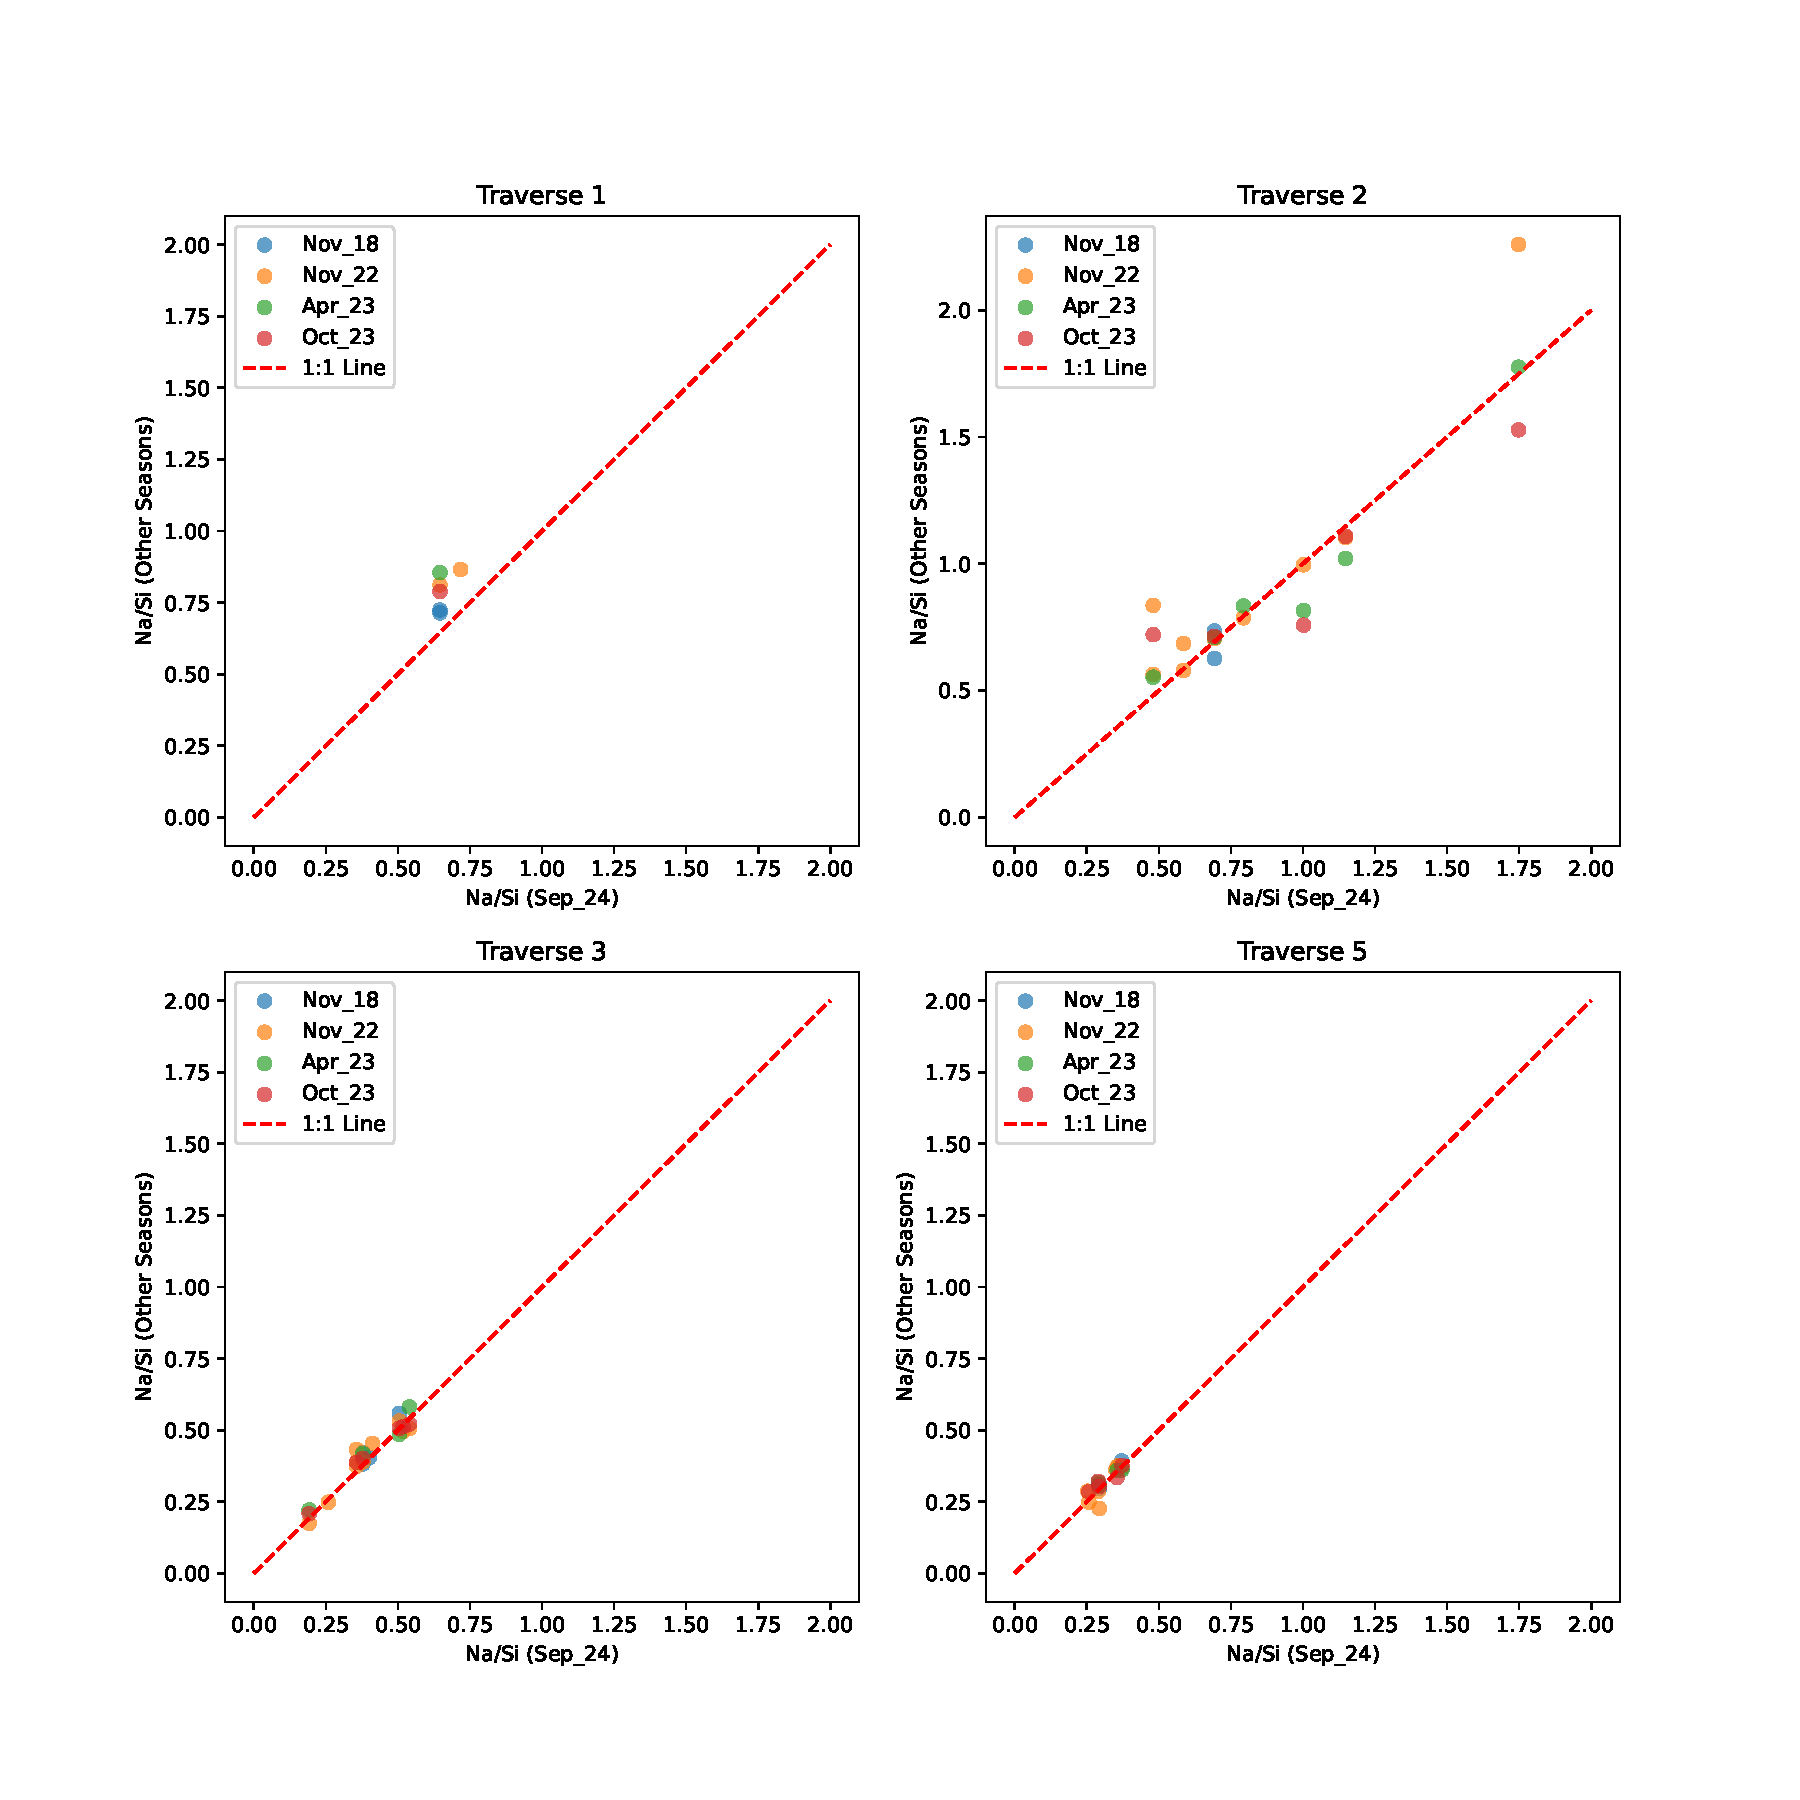
\includegraphics[width=\textwidth]{Na_Si_Seasons.pdf}
%     \caption{How Na/Si varies for different traverses. Traverse 4 is not plotted due to the lack of samples.}
%     \label{fig:spatial_changes_spring8}
% \end{figure}
% \FloatBarrier

% The scatter in these plots reflect temporal variability in the spring chemistry. Traverses 1 and 5 both display tight scatter, consistent with the notion that the flow paths here are consistently sampled. More notable here are the differences in Na/Si values between traverses. These how the spatial variability between traverses is more significant than the temporal variability. It is possible, and quite likely that all traverses flow paths are connected one to the other. When investigating model differences, however, a knowledge of which traverse accounts for what discrepancy allows for the contribution of spatial variation toward the overall interpretation to be taken into account.


% \subsection{Lithological Control on Spring Chemistry}

% Radiogenic strontium isotope analyses of springs show significant variation between different traverses. Sr isotope values of rain are consistent with the expected values for rainwater, with the exception of those sampled at low elevation (Galy, France-Lenord, Derry, 1999). The lowest Sr isotope value for rain is very close to the reported value for seawater, which is 0.70917 (Paytan et al, 2021). The rain samples with low strontium isotopic composition therefore indicate little contamination from dust or particles. Strontium isotope ratios used alongside strontium concentrations can be used to determine mixing between different endmembers (Faure, 1986; See Appendix). Plots of $\ddfrac{^{87}Sr}{^{86}Sr}$ against $\ddfrac{1}{Sr}$ that yield straight lines are indicative of mixing trends.


% \begin{figure}[p]
%     \centering
%     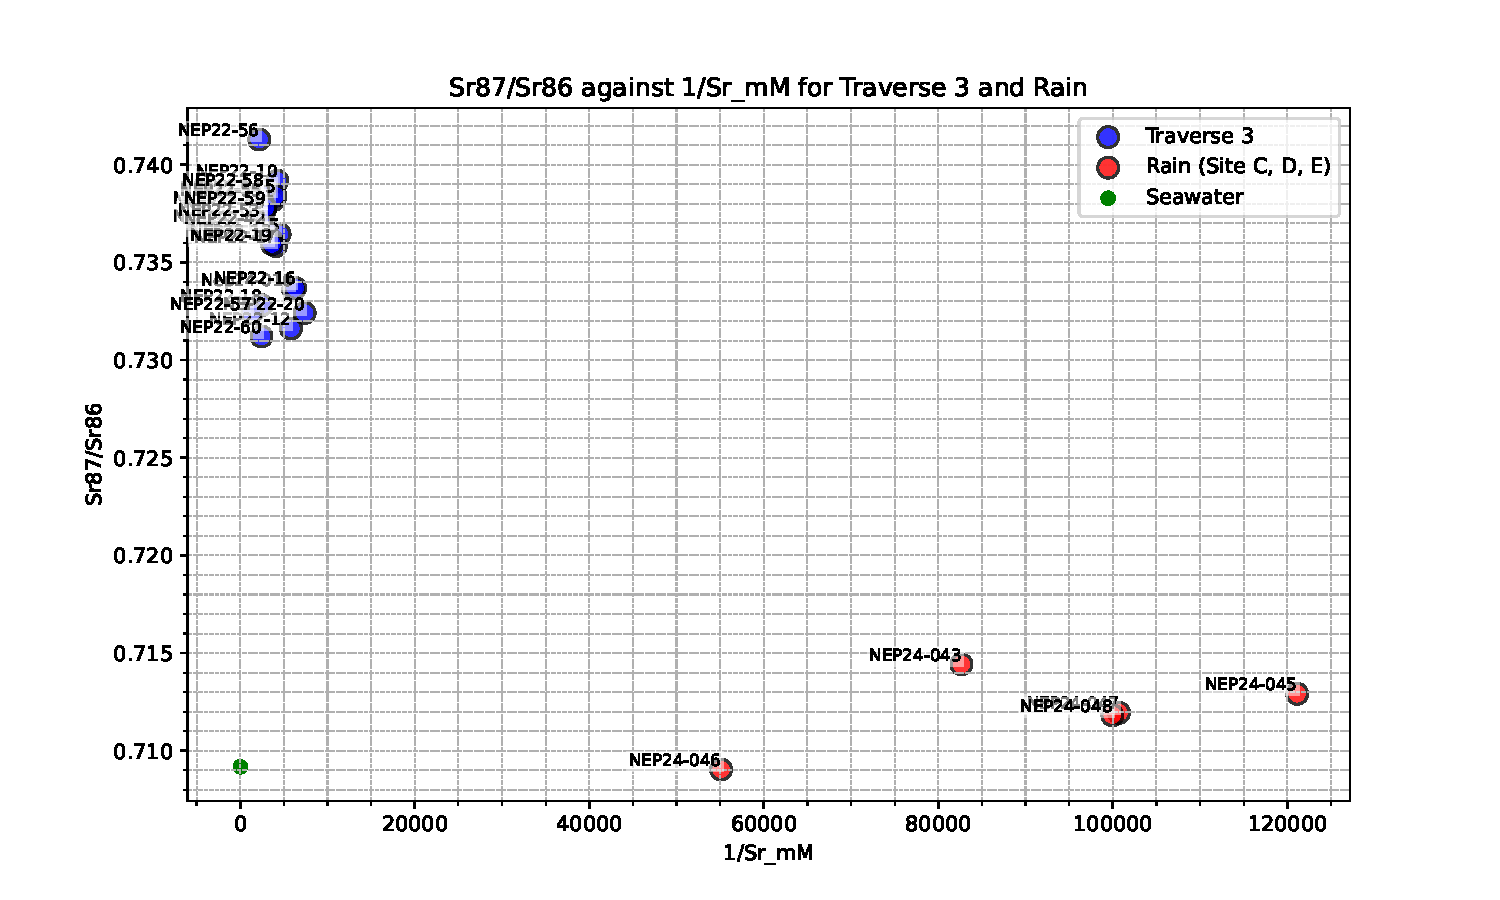
\includegraphics[width=\textwidth]{Sr87_Sr86_1Sr_Rain.pdf}
%     \caption{Strontium isotope differences display difference in lithology tapped in. Cite Quade and Tipper papers; Rain analysed for Sr isotopes and Cl. Something about contamination lower down; How samples of Traverse 3 compare to the rain samples}
%     \label{fig:discussion3}
% \end{figure}

% \FloatBarrier


% Comparing springs to rain in \ref{fig:discussion3}, the major control on spring chemistry does not appear to be the rain. Spring water mixing trends in $\ddfrac{^{87}Sr}{^{86}Sr}$ against $\ddfrac{1}{Sr}$ space are tightly scattered away from the rain. This suggests that rain input does not exert a significant control on the spring chemistry, which implies even the highest springs with the shortest flowpaths undergo significant weathering reactions with the rock. Instead, the water chemistry reflects that different traversal flowpaths sample lithologies that have different strontium isotopic composition. These variations are however within the range of Higher Himalayan Crystalline Series (HHCS) rocks found in the region, so this variation is to be expected (Tipper et al., 2006). It is unlikely that the source of the Sr isotopes is from the Lesser Himalayan Series (LHS) rocks, and the Main Central Thrust (MCT) is several km south of Melamchi.




\newpage




\section*{References}



\textbf{Remember to add a box explaining Sr isotopes in the Appendix}

Hello




\end{document}







%%  pdflatex Part3Report.tex && open Part3Report.pdf  